
\section{Experimente und Ergebnisse}

In diesem Kapitel wird der vorgeschlagene semi-supervisierte Ansatz zur automatischen Annotation von UAV-Videodaten experimentell untersucht. Ziel der Experimente ist es, zu bewerten, inwieweit ein auf sparsam annotierten Frames trainiertes YOLO-Modell zur automatischen Erweiterung des Trainingsdatensatzes eingesetzt werden kann. Der Fokus liegt dabei auf drei aufeinander aufbauenden experimentellen Stufen: dem initialen Baseline-Modell, der automatischen Pseudo-Label-Generierung sowie der tracking-basierten Label-Propagation.

Die folgenden Abschnitte beschreiben zunächst den experimentellen Aufbau, die verwendete Datenbasis, die eingesetzten Softwarekomponenten sowie die Struktur der untersuchten Experimente. Anschließend werden die Ergebnisse anhand der erzeugten Modellmetriken, Evaluationsgrafiken, Konfusionsmatrizen und qualitativen Validierungsbeispiele dargestellt.

\subsection{Experimenteller Aufbau}

Der experimentelle Aufbau orientiert sich an dem in Kapitel~5 beschriebenen methodischen Ablauf. Ausgangspunkt ist eine begrenzte Menge manuell annotierter Frames aus dem MBG-V2-Datensatz~\cite{passos2024mbgv2}. Diese Frames dienen zum initialen Training eines YOLO-basierten Objekterkennungsmodells mittels Transfer Learning. Anschließend wird das trainierte Modell auf nicht manuell annotierte Zwischenframes angewendet, um zusätzliche Annotationen in Form von Pseudo-Labels zu erzeugen. Ergänzend wird ein Tracking-Verfahren eingesetzt, um Detektionen über aufeinanderfolgende Frames hinweg zeitlich zu verknüpfen und für die Label-Propagation nutzbar zu machen.

Die Experimente sind so aufgebaut, dass der Einfluss der einzelnen Erweiterungen schrittweise untersucht werden kann. Zunächst wird ein Baseline-Modell ausschließlich auf den manuell annotierten Frames trainiert. Danach wird dieses Modell zur automatischen Erzeugung zusätzlicher Pseudo-Labels verwendet. In einem weiteren Schritt wird die zeitliche Struktur der Videodaten durch Objektverfolgung genutzt, um die erzeugten Labels über mehrere Frames hinweg zu stabilisieren.

Hardware-spezifische Laufzeitvergleiche stehen nicht im Fokus dieser Arbeit. Daher werden keine detaillierten Angaben zu Prozessor, Arbeitsspeicher oder Betriebssystem gemacht. Entscheidend für die Auswertung ist der Vergleich der untersuchten Annotationsstrategien unter konsistenten experimentellen Bedingungen.

\subsubsection{Datengrundlage der Experimente}

Als Datengrundlage dient der in Kapitel~3 beschriebene MBG-V2-Datensatz~\cite{passos2024mbgv2}. Der Datensatz besteht aus UAV-Videodaten urbaner Gebiete und enthält Annotationen potenzieller Brutstätten von \textit{Aedes aegypti}. Da die Annotationen ursprünglich track-basiert vorliegen, wurden sie zunächst in ein framebasiertes Format überführt und anschließend in das YOLO-Format konvertiert. Jede Label-Datei enthält dabei die Klassen-ID sowie die normalisierten Bounding-Box-Koordinaten des jeweiligen Objekts.

Die manuelle Annotation der ausgewählten Frames erfolgte mit dem Computer Vision Annotation Tool CVAT~\cite{cvat2024}. Für das initiale Training wurden ausschließlich die manuell annotierten Frames verwendet. Die dazwischenliegenden, zunächst unannotierten Frames wurden im weiteren Verlauf für die automatische Pseudo-Label-Generierung und die tracking-basierte Label-Propagation genutzt.

Dieses Vorgehen bildet ein realistisches Szenario ab, in dem nur ein begrenzter Teil der Videodaten manuell annotiert ist, während der größere Teil der Daten automatisch erschlossen werden soll. Dadurch kann untersucht werden, ob der manuelle Annotierungsaufwand durch die Kombination von Objekterkennung, Pseudo-Labeling und Tracking reduziert werden kann.

\subsubsection{Verwendete Software}

Für die Implementierung des vorgeschlagenen Verfahrens wurden etablierte Open-Source-Werkzeuge aus den Bereichen Deep Learning, Computer Vision und Multi-Object-Tracking verwendet. Das Training und die Inferenz des Objektdetektors erfolgten mit der Ultralytics-Implementierung von YOLOv8~\cite{Ultralytics2023}. Die Verarbeitung der Bild- und Videodaten, insbesondere die Frame-Extraktion und die weitere Datenaufbereitung, wurde mithilfe von Python-basierten Verarbeitungsschritten durchgeführt.

Für die tracking-basierte Verknüpfung der Detektionen wurde ByteTrack verwendet~\cite{bytetrack}. Dabei handelt es sich um ein Tracking-by-Detection-Verfahren, bei dem frameweise Detektionen über aufeinanderfolgende Frames hinweg zu konsistenten Objekttracks verbunden werden. Diese Objekttracks dienen im weiteren Verlauf als Grundlage für die tracking-basierte Label-Propagation.

\subsubsection{Struktur der Experimente}

Die experimentelle Untersuchung besteht aus drei aufeinander aufbauenden Stufen. Jede Stufe erweitert die vorherige um einen zusätzlichen Verarbeitungsschritt. Dadurch kann der Beitrag der einzelnen Komponenten des vorgeschlagenen Ansatzes getrennt betrachtet werden.

\begin{table}[htbp]
    \centering
    \caption{Übersicht der untersuchten experimentellen Stufen}
    \label{tab:experimentelle_stufen}
    \begin{tabular}{p{3.7cm}p{5.4cm}p{4.0cm}}
        \hline
        \textbf{Experiment}                 & \textbf{Verwendete Daten}                       & \textbf{Ziel}                             \\
        \hline
        Baseline-Modell                     & Manuell annotierte Frames                       & Referenzmodell                            \\
        Pseudo-Labeling                     & Manuelle Labels und automatisch erzeugte Labels & Erweiterung der Trainingsdaten            \\
        Tracking-basierte Label-Propagation & Manuelle Labels und tracking-basierte Labels    & Zeitliche Stabilisierung der Annotationen \\
        \hline
    \end{tabular}
\end{table}

Das Baseline-Modell dient als Referenz für die nachfolgenden Experimente. Es zeigt, welche Detektionsleistung allein auf Basis der sparsam vorhandenen manuellen Annotationen erreicht werden kann. Die Pseudo-Labeling-Stufe untersucht, ob das initial trainierte Modell zusätzliche Labels auf unannotierten Zwischenframes erzeugen kann. Die tracking-basierte Label-Propagation erweitert diesen Ansatz, indem zusätzlich die zeitliche Konsistenz der Videodaten genutzt wird.

\subsubsection{Bewertungsverfahren}

Die Bewertung der Modelle erfolgt anhand der in Abschnitt~2.3.3 beschriebenen Metriken Precision, Recall, mAP@50 und mAP@50--95. Diese Metriken erlauben eine quantitative Bewertung der Detektionsleistung sowie der Lokalisierungsqualität der vorhergesagten Bounding Boxes.

Zusätzlich werden die von YOLO erzeugten Evaluationsgrafiken ausgewertet. Dazu gehören die Trainingskurven, die Label-Verteilung, die Precision-Recall-Kurve, die F1-Confidence-Kurve sowie absolute und normalisierte Konfusionsmatrizen. Ergänzend werden qualitative Validierungsbeispiele betrachtet, bei denen Ground-Truth-Labels und Modellvorhersagen gegenübergestellt werden. Dadurch können typische Fehlerfälle wie False Positives, nicht erkannte Objekte und Verwechslungen mit dem Hintergrund sichtbar gemacht werden.

\subsection{Quantitative Ergebnisse des Baseline-Modells}

Das Baseline-Modell bildet die Referenz für alle weiteren Experimente. Es wurde ausschließlich auf den manuell annotierten Frames trainiert und zeigt damit, welche Detektionsleistung ohne zusätzliche automatisch erzeugte Labels erreicht werden kann. Die Auswertung dieses Modells ist besonders wichtig, da die Qualität der später erzeugten Pseudo-Labels direkt von der Leistungsfähigkeit dieses initialen Modells abhängt. Fehler des Baseline-Modells können sich im semi-supervisierten Schritt in den erweiterten Trainingsdatensatz übertragen und dort verstärken.

Die Ergebnisse werden daher nicht nur anhand globaler Kennzahlen wie mAP@50, Precision und Recall bewertet, sondern zusätzlich über die Klassenverteilung, die Precision-Recall-Kurve, die F1-Confidence-Kurve, die Konfusionsmatrizen und qualitative Validierungsbeispiele analysiert. Dadurch lässt sich nachvollziehen, welche Objektklassen bereits zuverlässig erkannt werden und bei welchen Klassen die begrenzte Menge manueller Annotationen zu instabilen Vorhersagen führt.

\subsubsection{Trainingsverlauf des Baseline-Modells}

Die Trainings- und Validierungsmetriken des Baseline-Modells sind in Abbildung~\ref{fig:baseline_results} dargestellt. Die Loss-Verläufe zeigen, dass das Modell während des Trainings grundsätzlich konvergiert. Sowohl der Box-Loss als auch der Klassifikations-Loss nehmen im Verlauf der Epochen ab. Dies deutet darauf hin, dass das Modell zunehmend bessere räumliche Lokalisierungen und stabilere Klassenzuordnungen lernt.

Auffällig ist jedoch, dass die Validierungsmetriken stärker schwanken als die geglätteten Trainingskurven. Dies ist ein Hinweis darauf, dass die verfügbare Menge an manuell annotierten Validierungsdaten begrenzt ist und einzelne schwierigere Frames einen sichtbaren Einfluss auf die Metriken haben können. Besonders bei UAV-Aufnahmen mit kleinen Objekten, dichten Dachstrukturen und variierenden Beleuchtungsbedingungen kann bereits eine geringe Anzahl falsch lokalisierter Objekte zu deutlichen Schwankungen in Recall und mAP führen.

Die Precision steigt im Verlauf des Trainings deutlich an und erreicht in der letzten Trainingsphase Werte von ungefähr 0{,}85. Der Recall bleibt dagegen niedriger und liegt zuletzt bei ungefähr 0{,}53. Diese Kombination zeigt, dass das Modell bei seinen Vorhersagen vergleichsweise zuverlässig ist, jedoch weiterhin einen relevanten Teil der vorhandenen Objekte nicht erkennt. Für die spätere automatische Annotation bedeutet dies, dass das Baseline-Modell eher konservativ arbeitet: erkannte Objekte sind häufig plausibel, aber nicht alle potenziellen Objekte werden vollständig erfasst.

\begin{figure}[htbp]
    \centering
    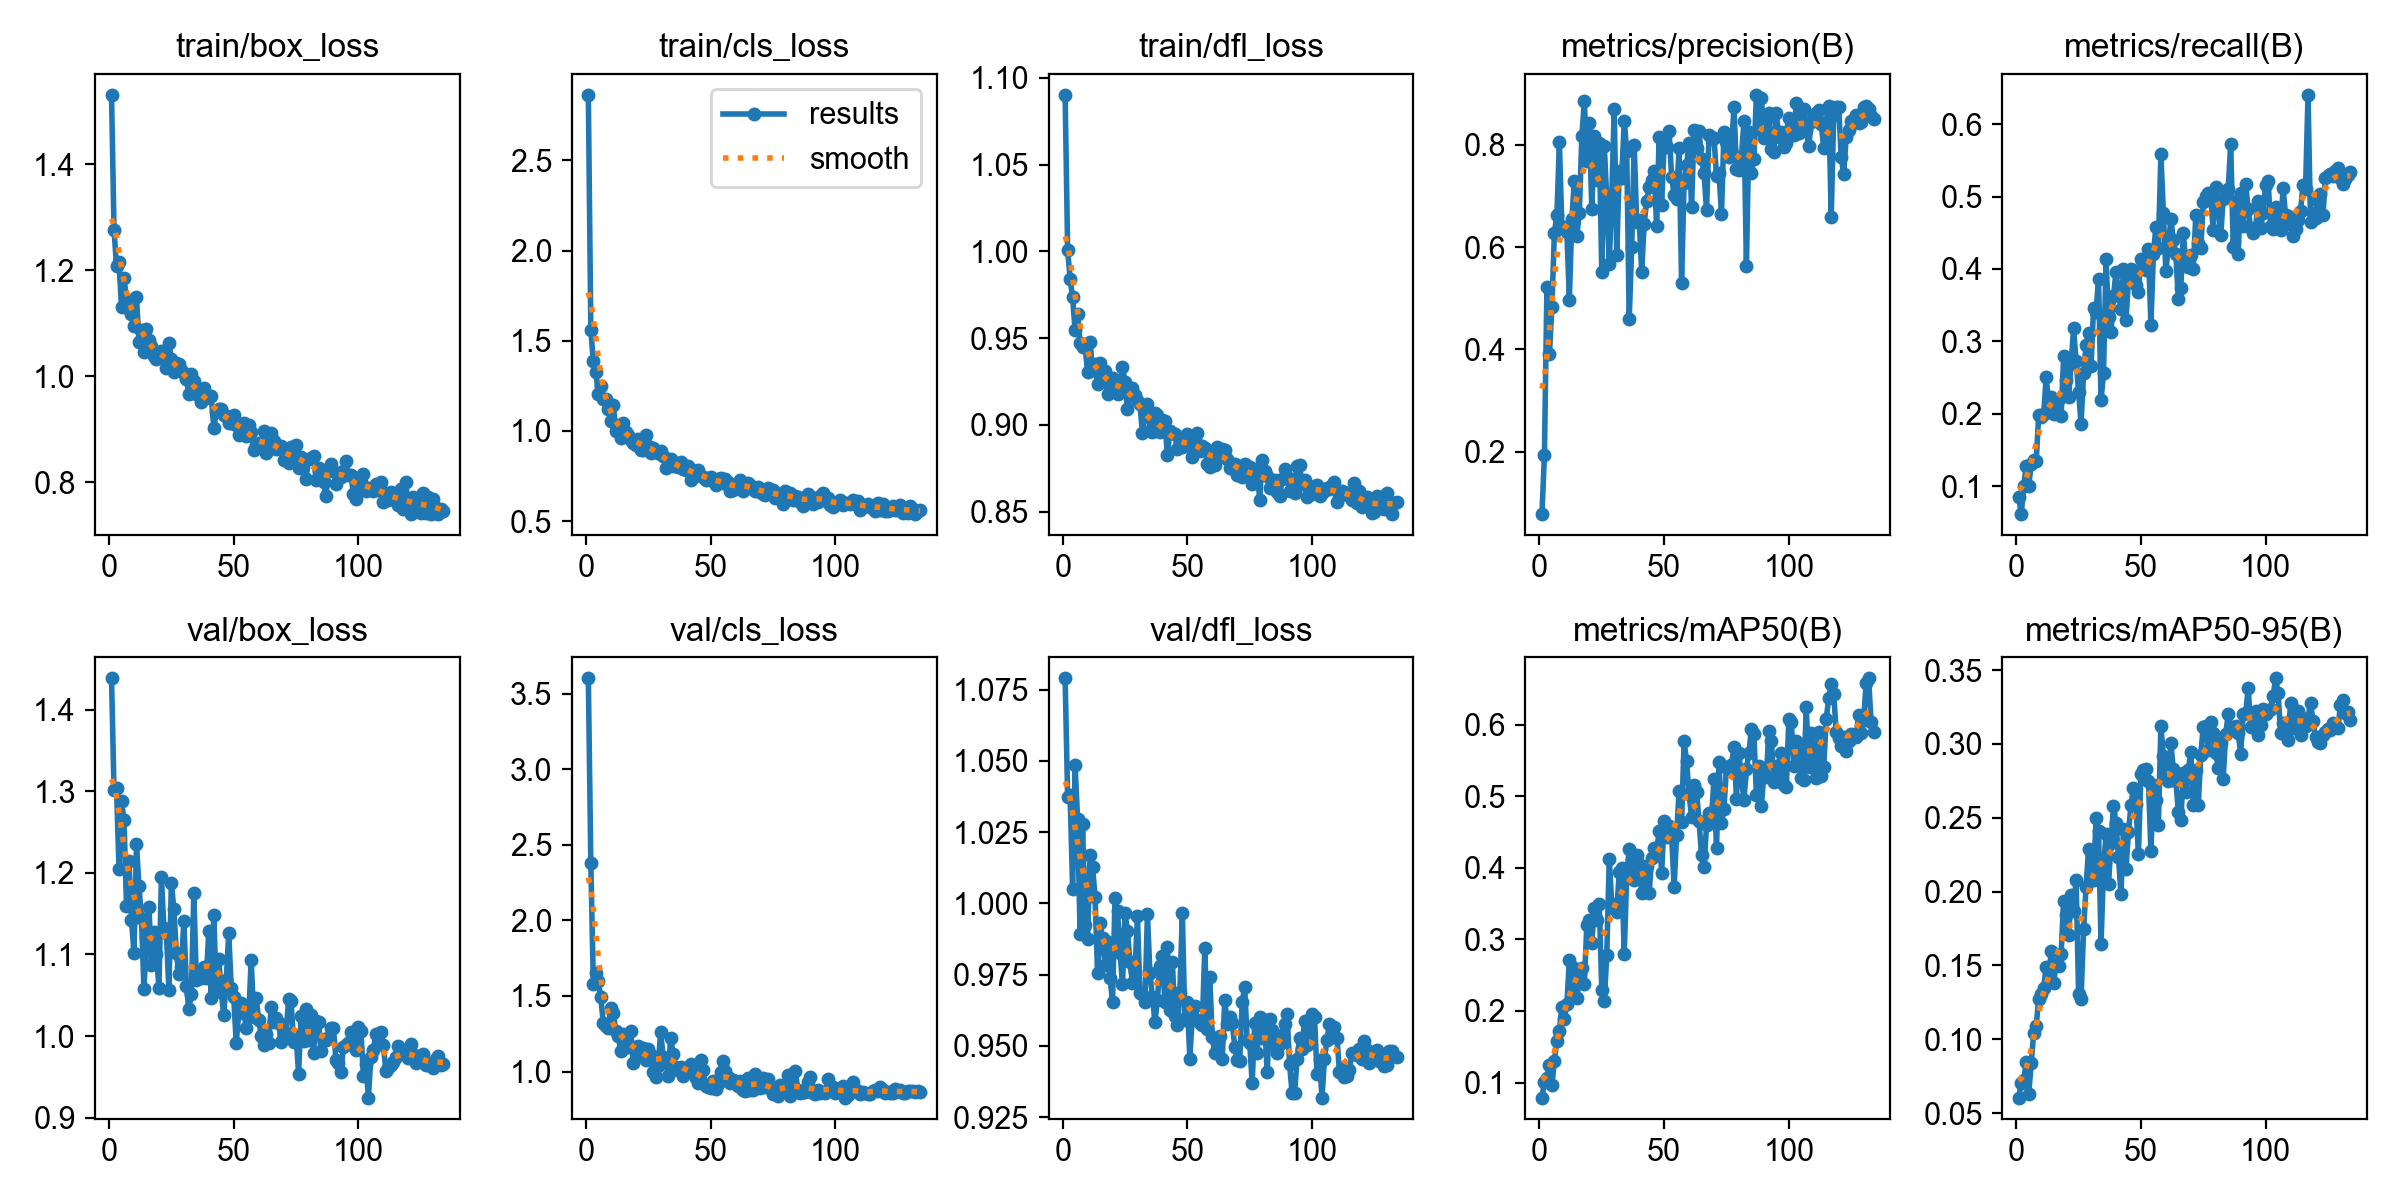
\includegraphics[width=\textwidth]{figures/baseline/results.png}
    \caption{Trainings- und Validierungsmetriken des Baseline-Modells. Dargestellt sind die Loss-Verläufe sowie Precision, Recall, mAP@50 und mAP@50--95.}
    \label{fig:baseline_results}
\end{figure}

\subsubsection{Daten- und Klassenverteilung}

Eine zentrale Ursache für die unterschiedlichen Klassenleistungen ist die stark unausgewogene Label-Verteilung im Trainingsdatensatz. Diese Verteilung ist in Abbildung~\ref{fig:baseline_labels} dargestellt. Die Klasse \textit{watertank} dominiert mit 4432 Instanzen deutlich. Im Vergleich dazu sind mehrere Klassen nur sehr schwach vertreten. Beispielsweise enthält die Klasse \textit{bottle} lediglich 14 Instanzen, \textit{plastic bag} 24 Instanzen und \textit{large trash bin} 43 Instanzen. Die Klasse \textit{puddle} ist im verwendeten Trainingssplit gar nicht vertreten und kann daher nicht sinnvoll bewertet werden.

\begin{figure}[htbp]
    \centering
    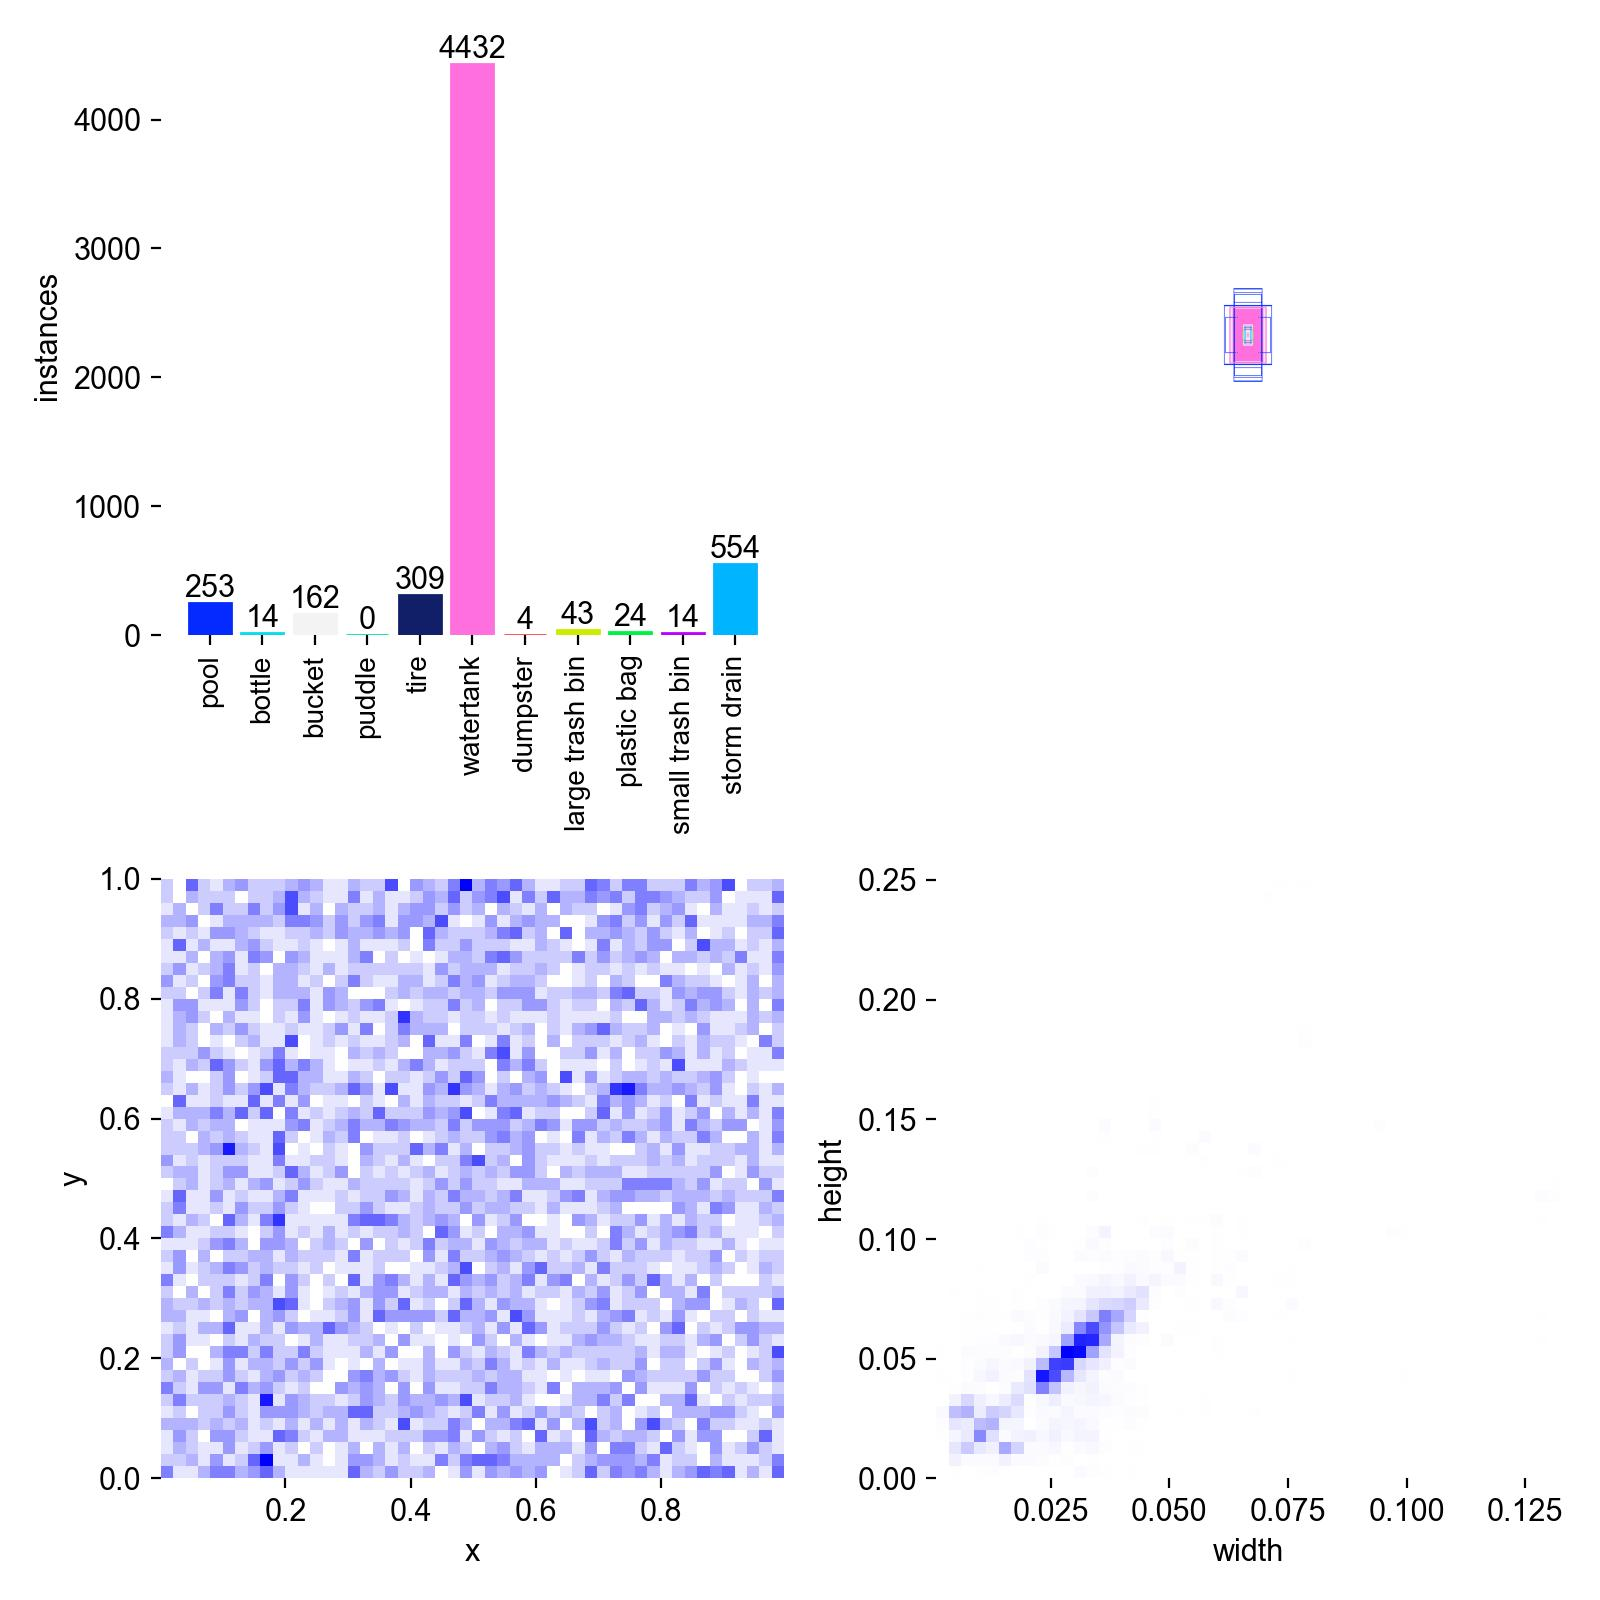
\includegraphics[width=0.85\textwidth]{figures/baseline/labels.jpg}
    \caption{Label-Verteilung und Bounding-Box-Verteilung im Baseline-Datensatz. Die starke Dominanz der Klasse \textit{watertank} ist deutlich erkennbar.}
    \label{fig:baseline_labels}
\end{figure}

\begin{table}[htbp]
    \centering
    \caption{Label-Verteilung im Baseline-Datensatz}
    \label{tab:baseline_labelverteilung}
    \begin{tabular}{lr}
        \hline
        \textbf{Klasse} & \textbf{Anzahl der Instanzen} \\
        \hline
        pool            & 253                           \\
        bottle          & 14                            \\
        bucket          & 162                           \\
        puddle          & 0                             \\
        tire            & 309                           \\
        watertank       & 4432                          \\
        dumpster        & 4                             \\
        large trash bin & 43                            \\
        plastic bag     & 24                            \\
        small trash bin & 14                            \\
        storm drain     & 554                           \\
        \hline
    \end{tabular}
\end{table}

Aufgrund der sehr geringen Anzahl an Trainingsbeispielen konnten insbesondere die Klassen \textit{dumpster} (4 Instanzen), \textit{small trash bin} (14 Instanzen) und \textit{puddle} (0 Instanzen) nicht zuverlässig gelernt werden. Zusätzlich erschweren ihre geringe Objektgröße sowie die starke visuelle Ähnlichkeit zum Hintergrund eine robuste Detektion. Aus diesem Grund werden die Ergebnisse dieser Klassen in der nachfolgenden Analyse nicht gesondert interpretiert.

\subsubsection{Detektionsleistung nach Klassen}

Die Precision-Recall-Kurve des Baseline-Modells ist in Abbildung~\ref{fig:baseline_pr_curve} dargestellt. Über alle Klassen hinweg wird ein mAP@50-Wert von 0{,}545 erreicht. Besonders gute Ergebnisse werden für die Klassen \textit{pool} und \textit{watertank} erzielt. Für \textit{pool} liegt der AP@50-Wert bei 0{,}866, für \textit{watertank} bei 0{,}737. Auch \textit{storm drain} erreicht mit 0{,}565 einen mittleren Wert. Schwächere Ergebnisse ergeben sich dagegen für Klassen mit geringer Anzahl an Trainingsinstanzen, insbesondere \textit{bucket}, \textit{tire}, \textit{large trash bin}, \textit{plastic bag} und \textit{bottle}.

\begin{figure}[htbp]
    \centering
    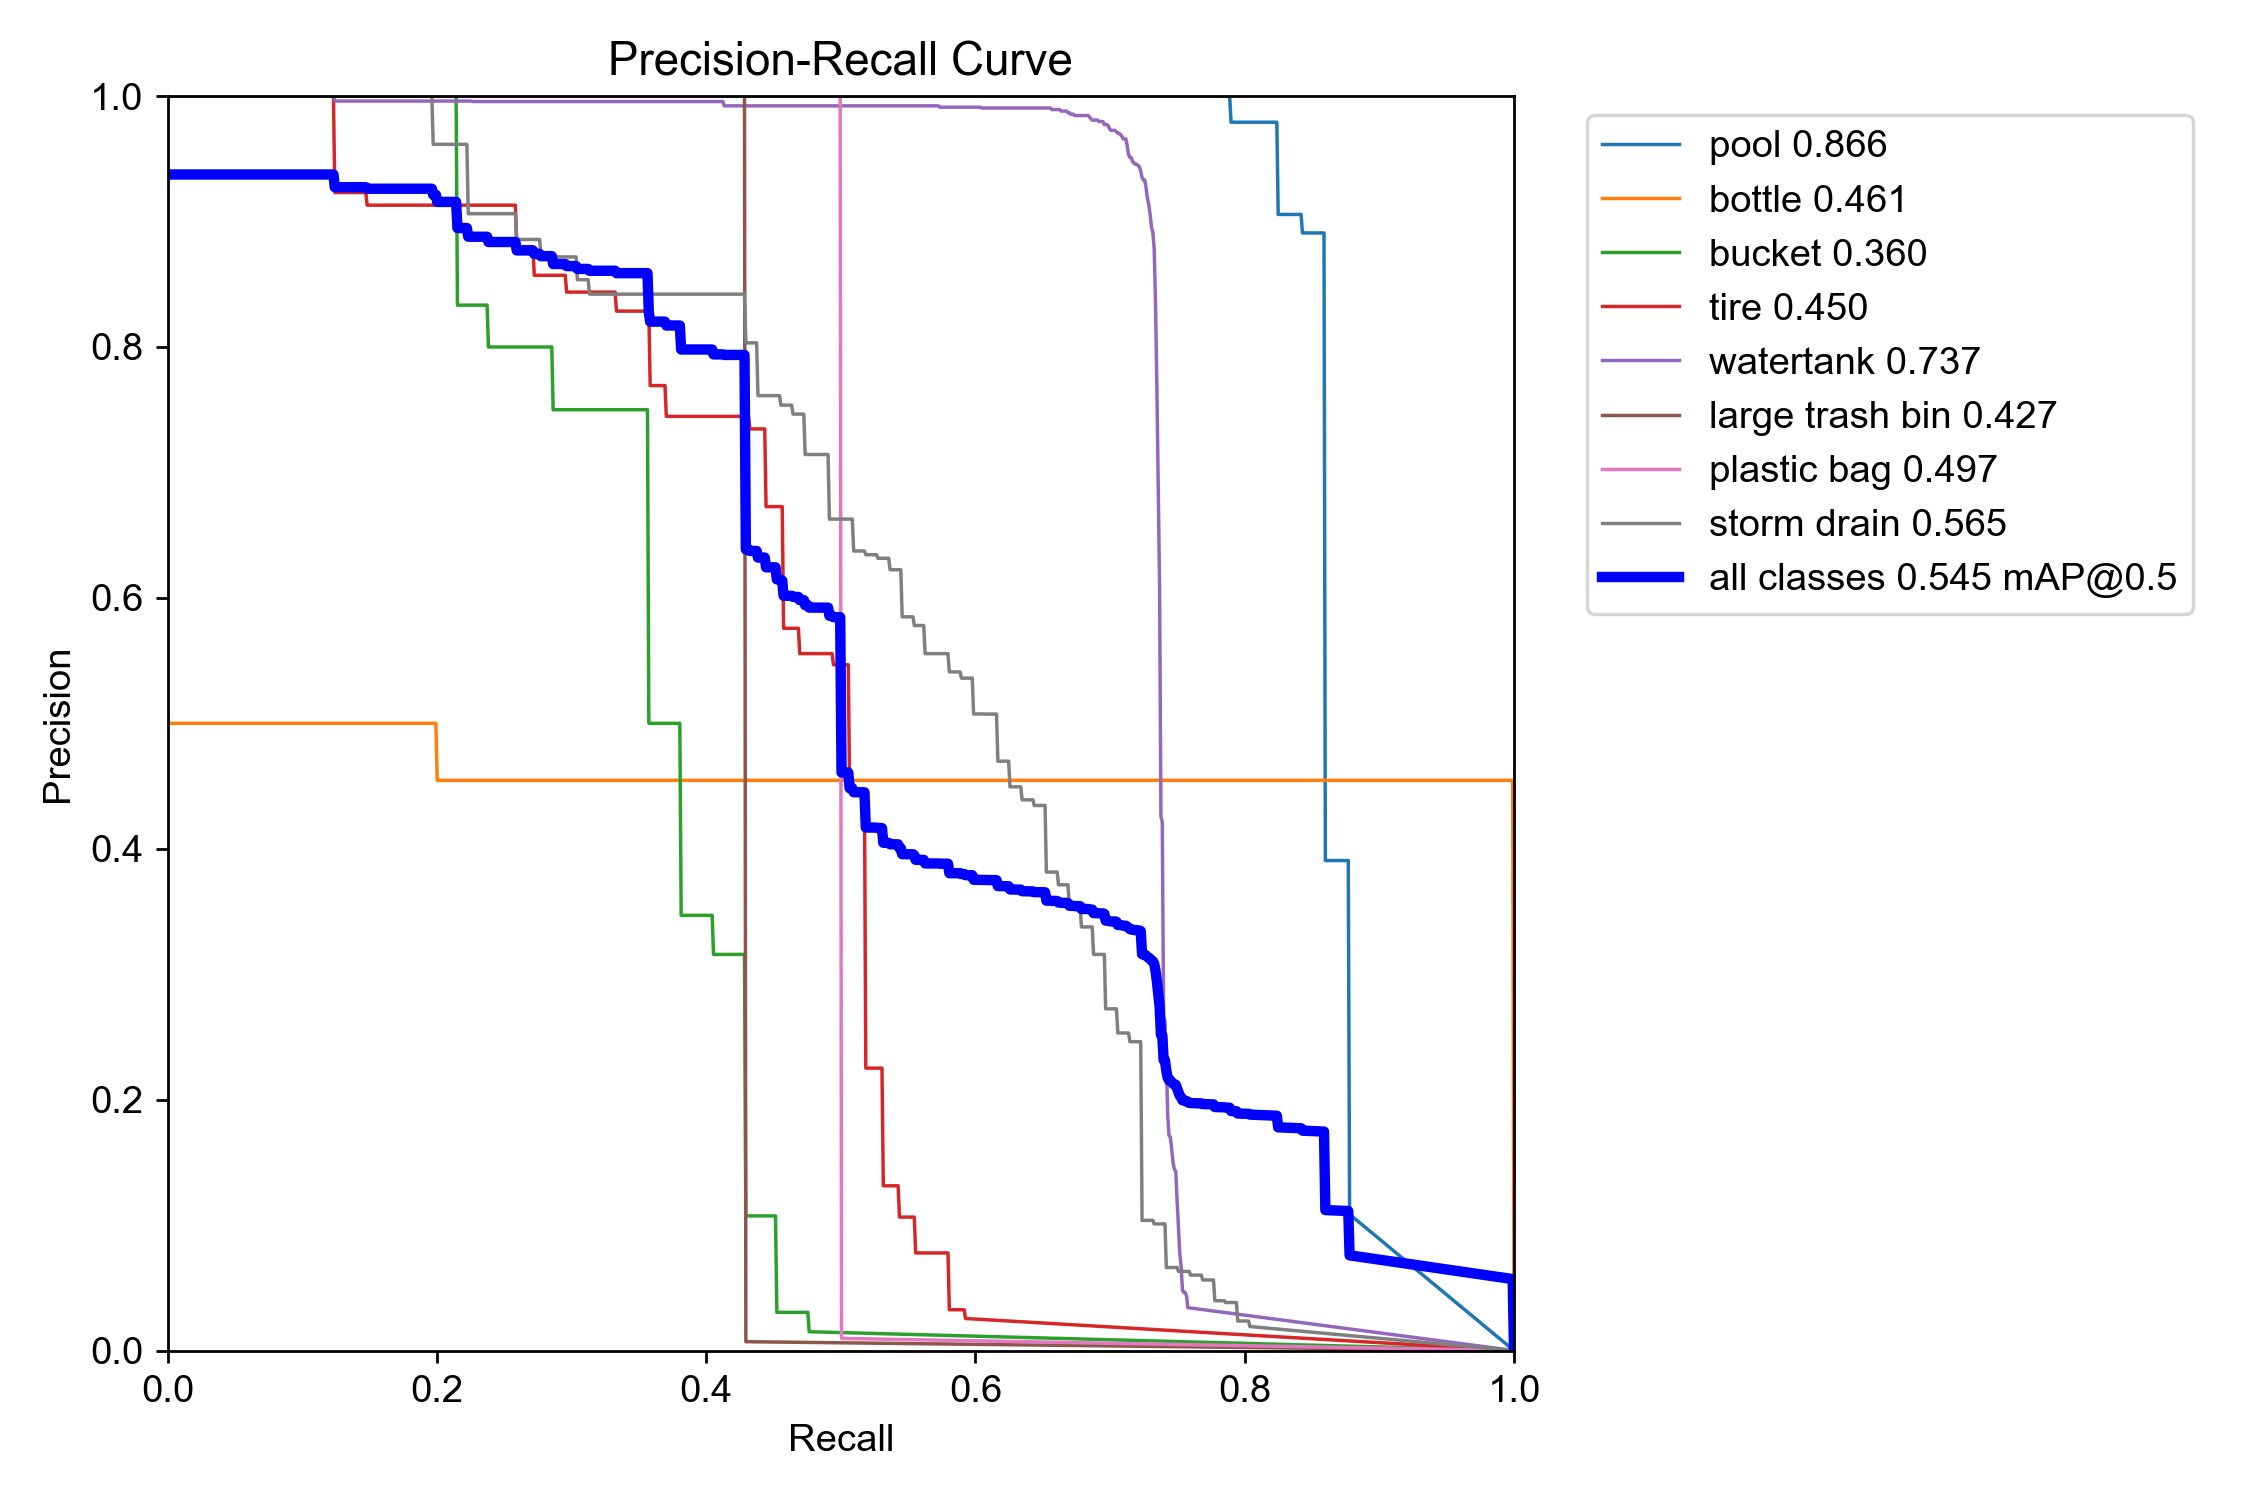
\includegraphics[width=0.9\textwidth]{figures/baseline/BoxPR_curve.png}
    \caption{Precision-Recall-Kurve des Baseline-Modells. Das Modell erreicht über alle Klassen einen mAP@50-Wert von 0{,}545.}
    \label{fig:baseline_pr_curve}
\end{figure}

\begin{table}[htbp]
    \centering
    \caption{Klassenweise AP@50-Werte des Baseline-Modells}
    \label{tab:baseline_ap_klassen}
    \begin{tabular}{lr}
        \hline
        \textbf{Klasse} & \textbf{AP@50} \\
        \hline
        pool            & 0{,}866        \\
        bottle          & 0{,}461        \\
        bucket          & 0{,}360        \\
        tire            & 0{,}450        \\
        watertank       & 0{,}737        \\
        large trash bin & 0{,}427        \\
        plastic bag     & 0{,}497        \\
        storm drain     & 0{,}565        \\
        \hline
        alle Klassen    & 0{,}545        \\
        \hline
    \end{tabular}
\end{table}

\subsubsection{Confidence-Schwellenwert und F1-Verhalten}

Die F1-Confidence-Kurve in Abbildung~\ref{fig:baseline_f1_curve} zeigt den Zusammenhang zwischen Confidence-Schwellenwert und F1-Wert. Der beste globale F1-Wert liegt bei etwa 0{,}53 und wird bei einem Confidence-Schwellenwert von ungefähr 0{,}462 erreicht. Dieser Wert beschreibt den besten Kompromiss zwischen Precision und Recall für das Baseline-Modell. Das Modell erzielt somit eine solide Ausgangsleistung, zeigt jedoch insbesondere beim Recall noch Einschränkungen.

\begin{figure}[htbp]
    \centering
    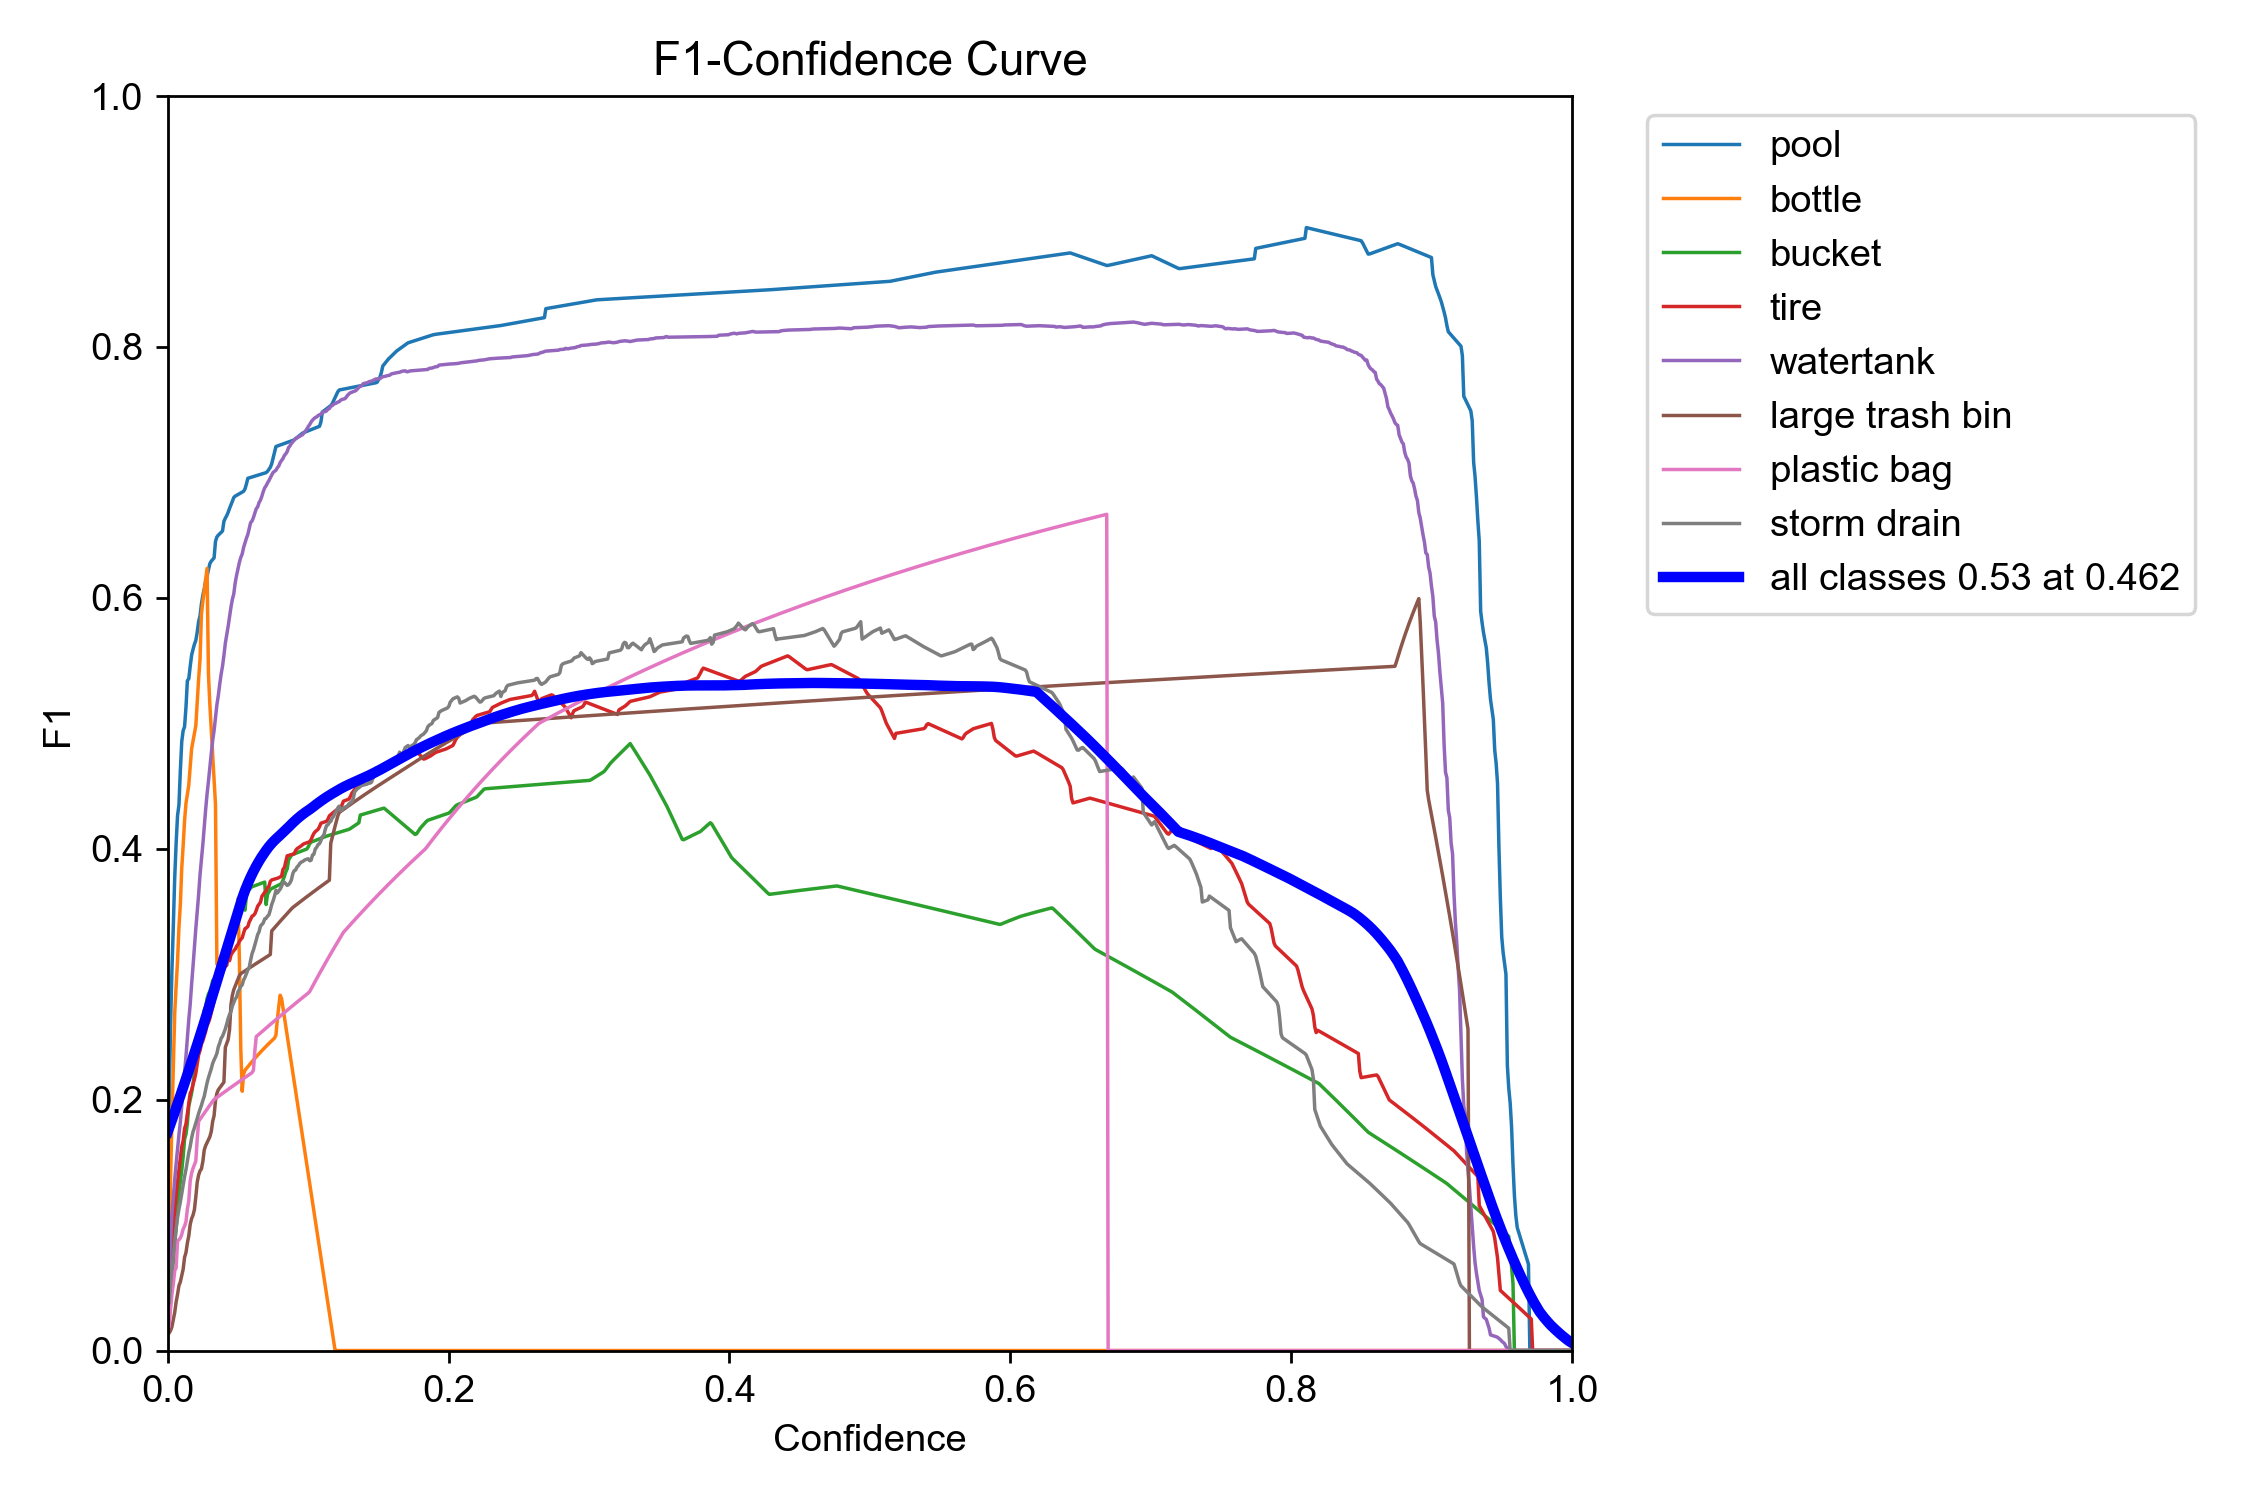
\includegraphics[width=0.9\textwidth]{figures/baseline/BoxF1_curve.png}
    \caption{F1-Confidence-Kurve des Baseline-Modells. Der beste globale F1-Wert liegt bei etwa 0{,}53 bei einem Confidence-Schwellenwert von 0{,}462.}
    \label{fig:baseline_f1_curve}
\end{figure}

\begin{table}[htbp]
    \centering
    \caption{Zusammenfassung der wichtigsten Kennzahlen des Baseline-Modells}
    \label{tab:baseline_kennzahlen}
    \begin{tabular}{lr}
        \hline
        \textbf{Metrik}                    & \textbf{Wert} \\
        \hline
        mAP@50, alle Klassen               & 0{,}545       \\
        F1-Wert, alle Klassen              & 0{,}53        \\
        optimaler Confidence-Schwellenwert & 0{,}462       \\
        Precision, letzte Trainingsphase   & ca. 0{,}85    \\
        Recall, letzte Trainingsphase      & ca. 0{,}53    \\
        \hline
    \end{tabular}
\end{table}

\subsubsection{Fehleranalyse anhand der Konfusionsmatrix}

Die absolute und die normalisierte Konfusionsmatrix des Baseline-Modells sind in Abbildung~\ref{fig:baseline_confusion_matrix} und Abbildung~\ref{fig:baseline_confusion_matrix_normalized} dargestellt. Sie zeigen, dass die Modellfehler weniger durch Verwechslungen zwischen vielen Objektklassen, sondern vor allem durch Verwechslungen mit dem Hintergrund geprägt sind. Dies ist für UAV-basierte Objekterkennung ein typisches Problem, da viele Zielobjekte sehr klein sind und sich visuell nur schwach von Dachflächen, Schatten, technischen Strukturen oder Straßenbereichen unterscheiden.

Die Klasse \textit{pool} wird mit 49 korrekt erkannten Instanzen vergleichsweise zuverlässig erkannt. Dies ist plausibel, da Pools in den Luftaufnahmen häufig eine klare Farbe, größere Fläche und gut abgegrenzte Form besitzen. Auch \textit{watertank} wird mit 817 korrekt erkannten Instanzen stark repräsentiert. Gleichzeitig zeigt die Matrix jedoch, dass 295 tatsächliche \textit{watertank}-Instanzen als Hintergrund gewertet werden. Das bedeutet, dass trotz hoher absoluter Trefferzahl ein relevanter Anteil der Wassertanks nicht erkannt wird.

Bei seltenen Klassen ist die Situation kritischer. Beispielsweise werden alle \textit{bottle}-Instanzen in der dargestellten Auswertung dem Hintergrund zugeordnet. Auch bei \textit{bucket}, \textit{tire}, \textit{large trash bin} und \textit{plastic bag} ist erkennbar, dass ein erheblicher Teil der tatsächlichen Objekte nicht detektiert wird. Der begrenzte Recall des Baseline-Modells entsteht somit nicht primär durch falsche Klassenzuordnungen zwischen Objektklassen, sondern durch übersehene Objekte.

Diese Beobachtung ist für die nachfolgende Pseudo-Label-Generierung entscheidend. Ein Modell mit gutem Precision-Verhalten, aber begrenztem Recall kann zwar relativ saubere Pseudo-Labels für sicher erkannte Objekte erzeugen, es wird jedoch viele schwer erkennbare oder seltene Objekte nicht automatisch ergänzen. Dadurch besteht die Gefahr, dass die ohnehin unausgewogene Klassenverteilung nur teilweise verbessert wird.

\begin{figure}[htbp]
    \centering
    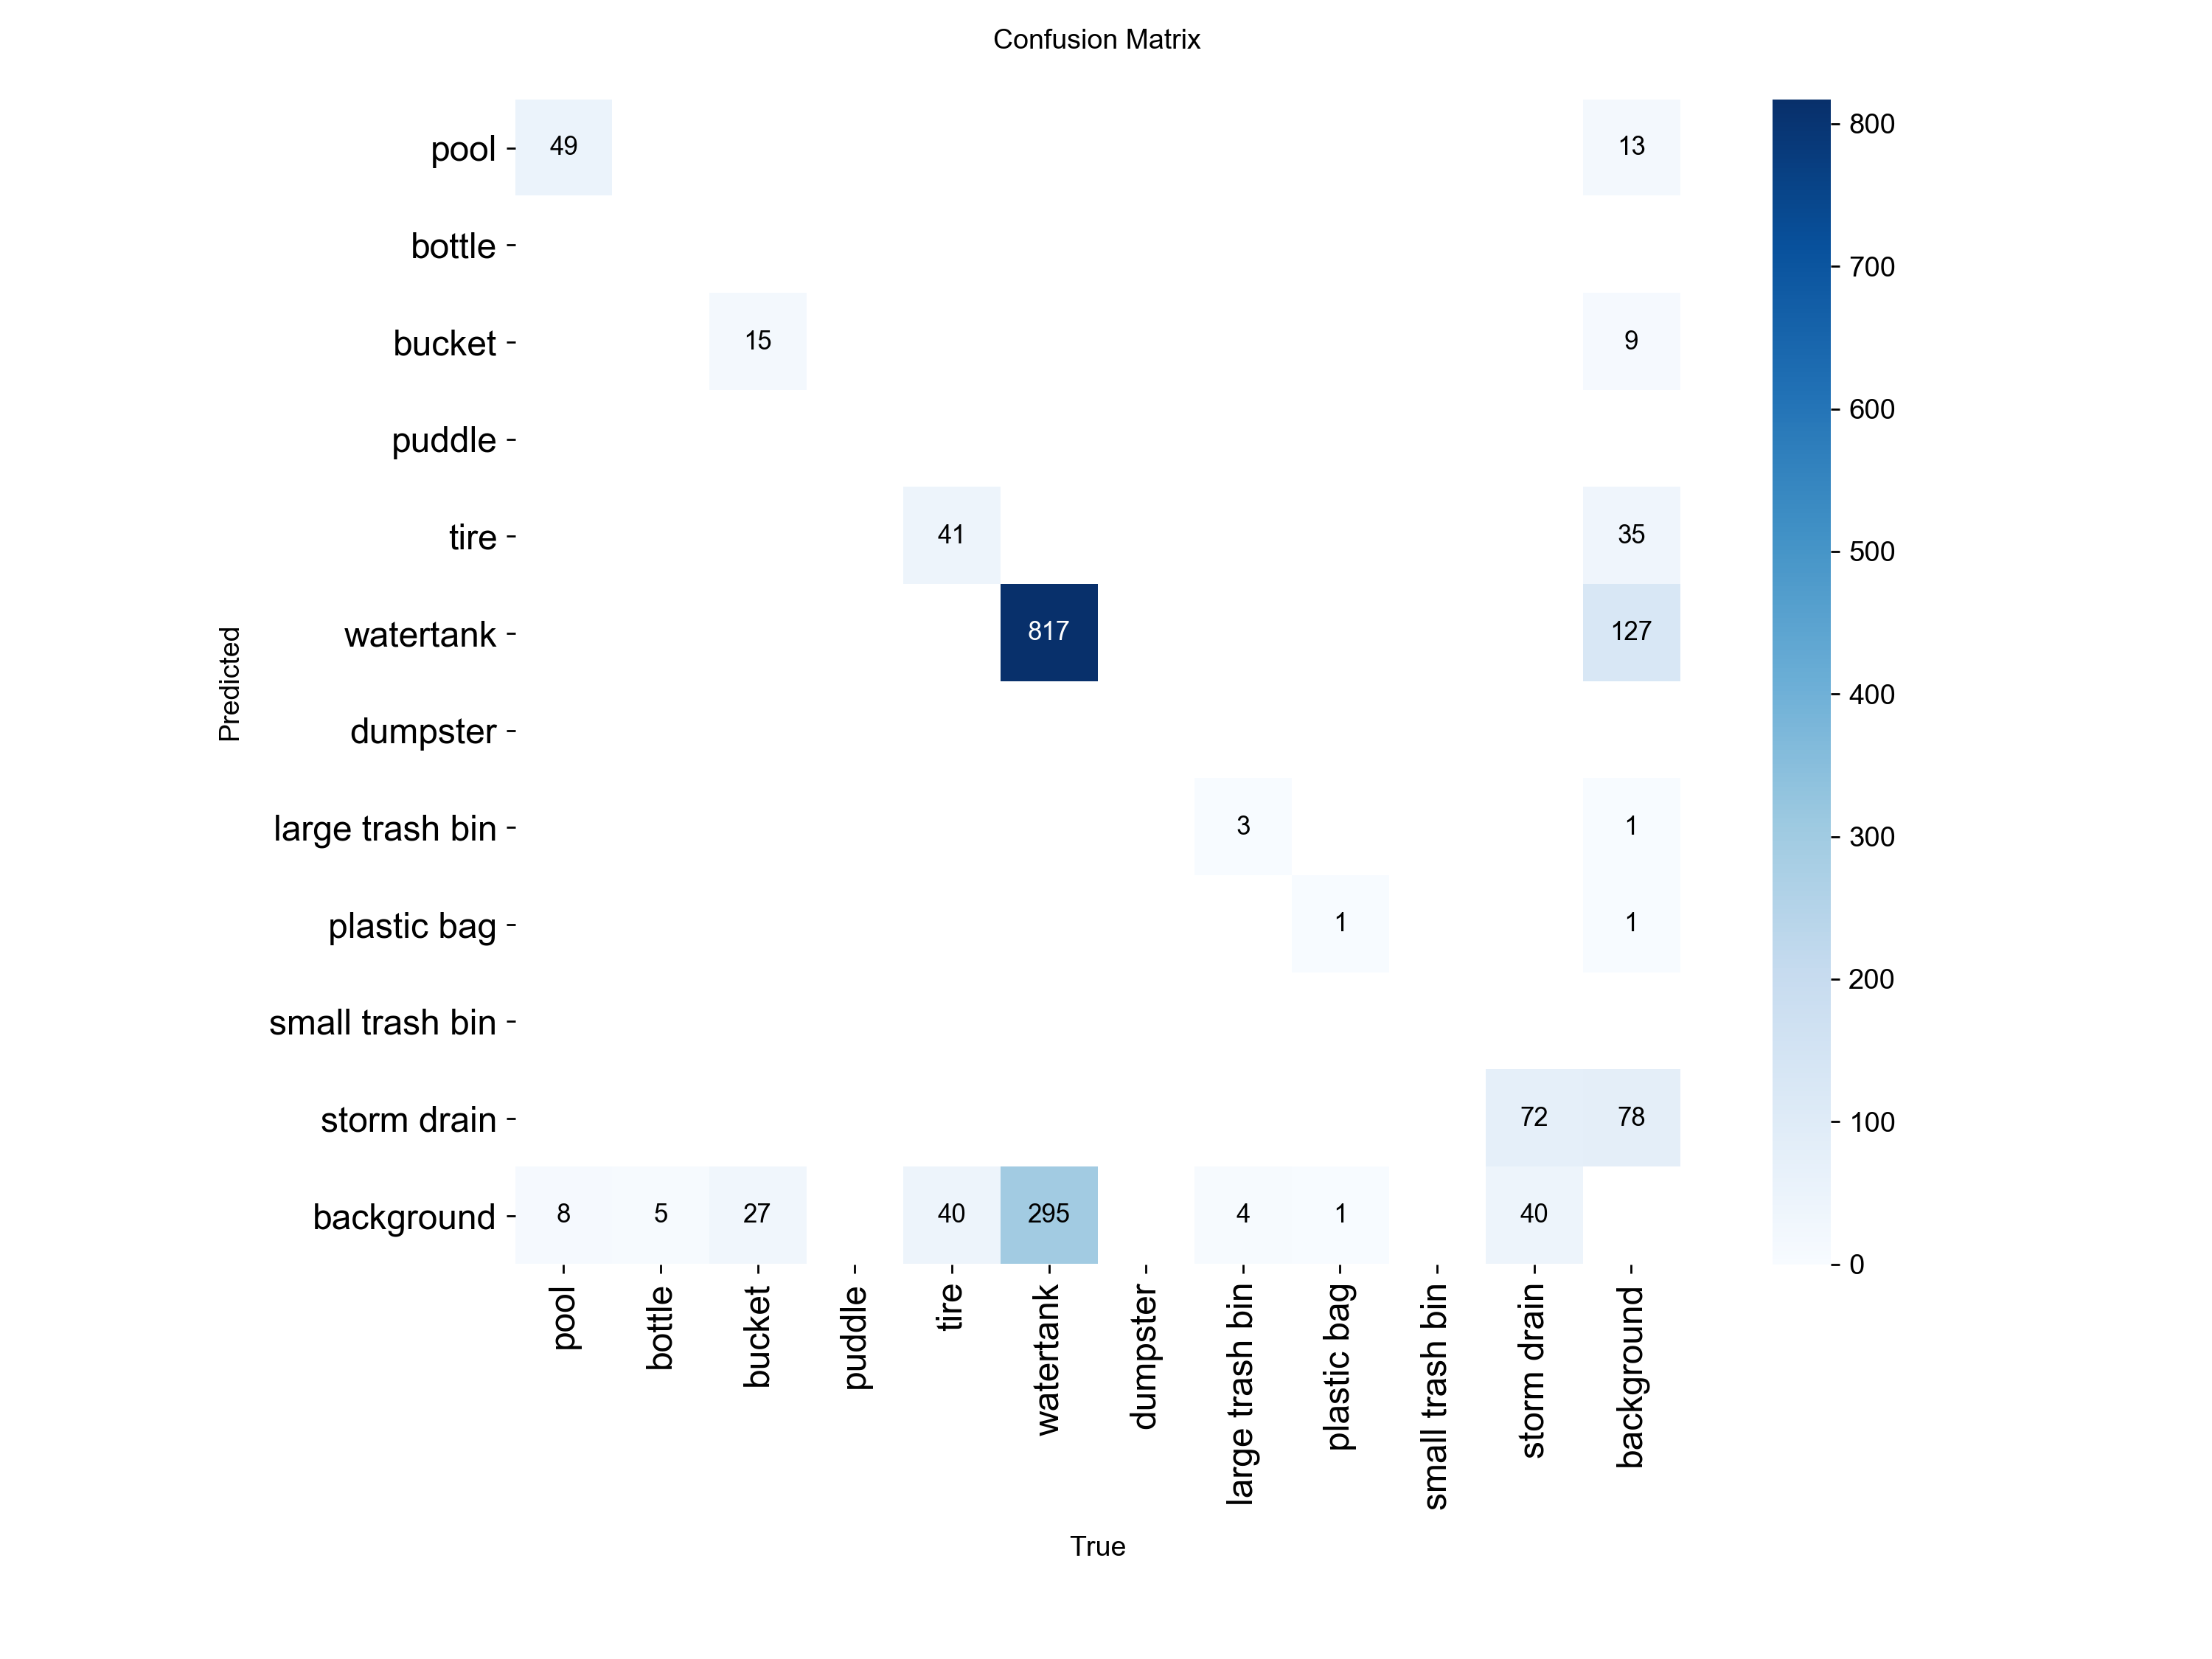
\includegraphics[width=0.9\textwidth]{figures/baseline/confusion_matrix.png}
    \caption{Absolute Konfusionsmatrix des Baseline-Modells. Die Matrix zeigt korrekte Vorhersagen sowie Fehlklassifikationen und nicht erkannte Objekte.}
    \label{fig:baseline_confusion_matrix}
\end{figure}

\begin{figure}[htbp]
    \centering
    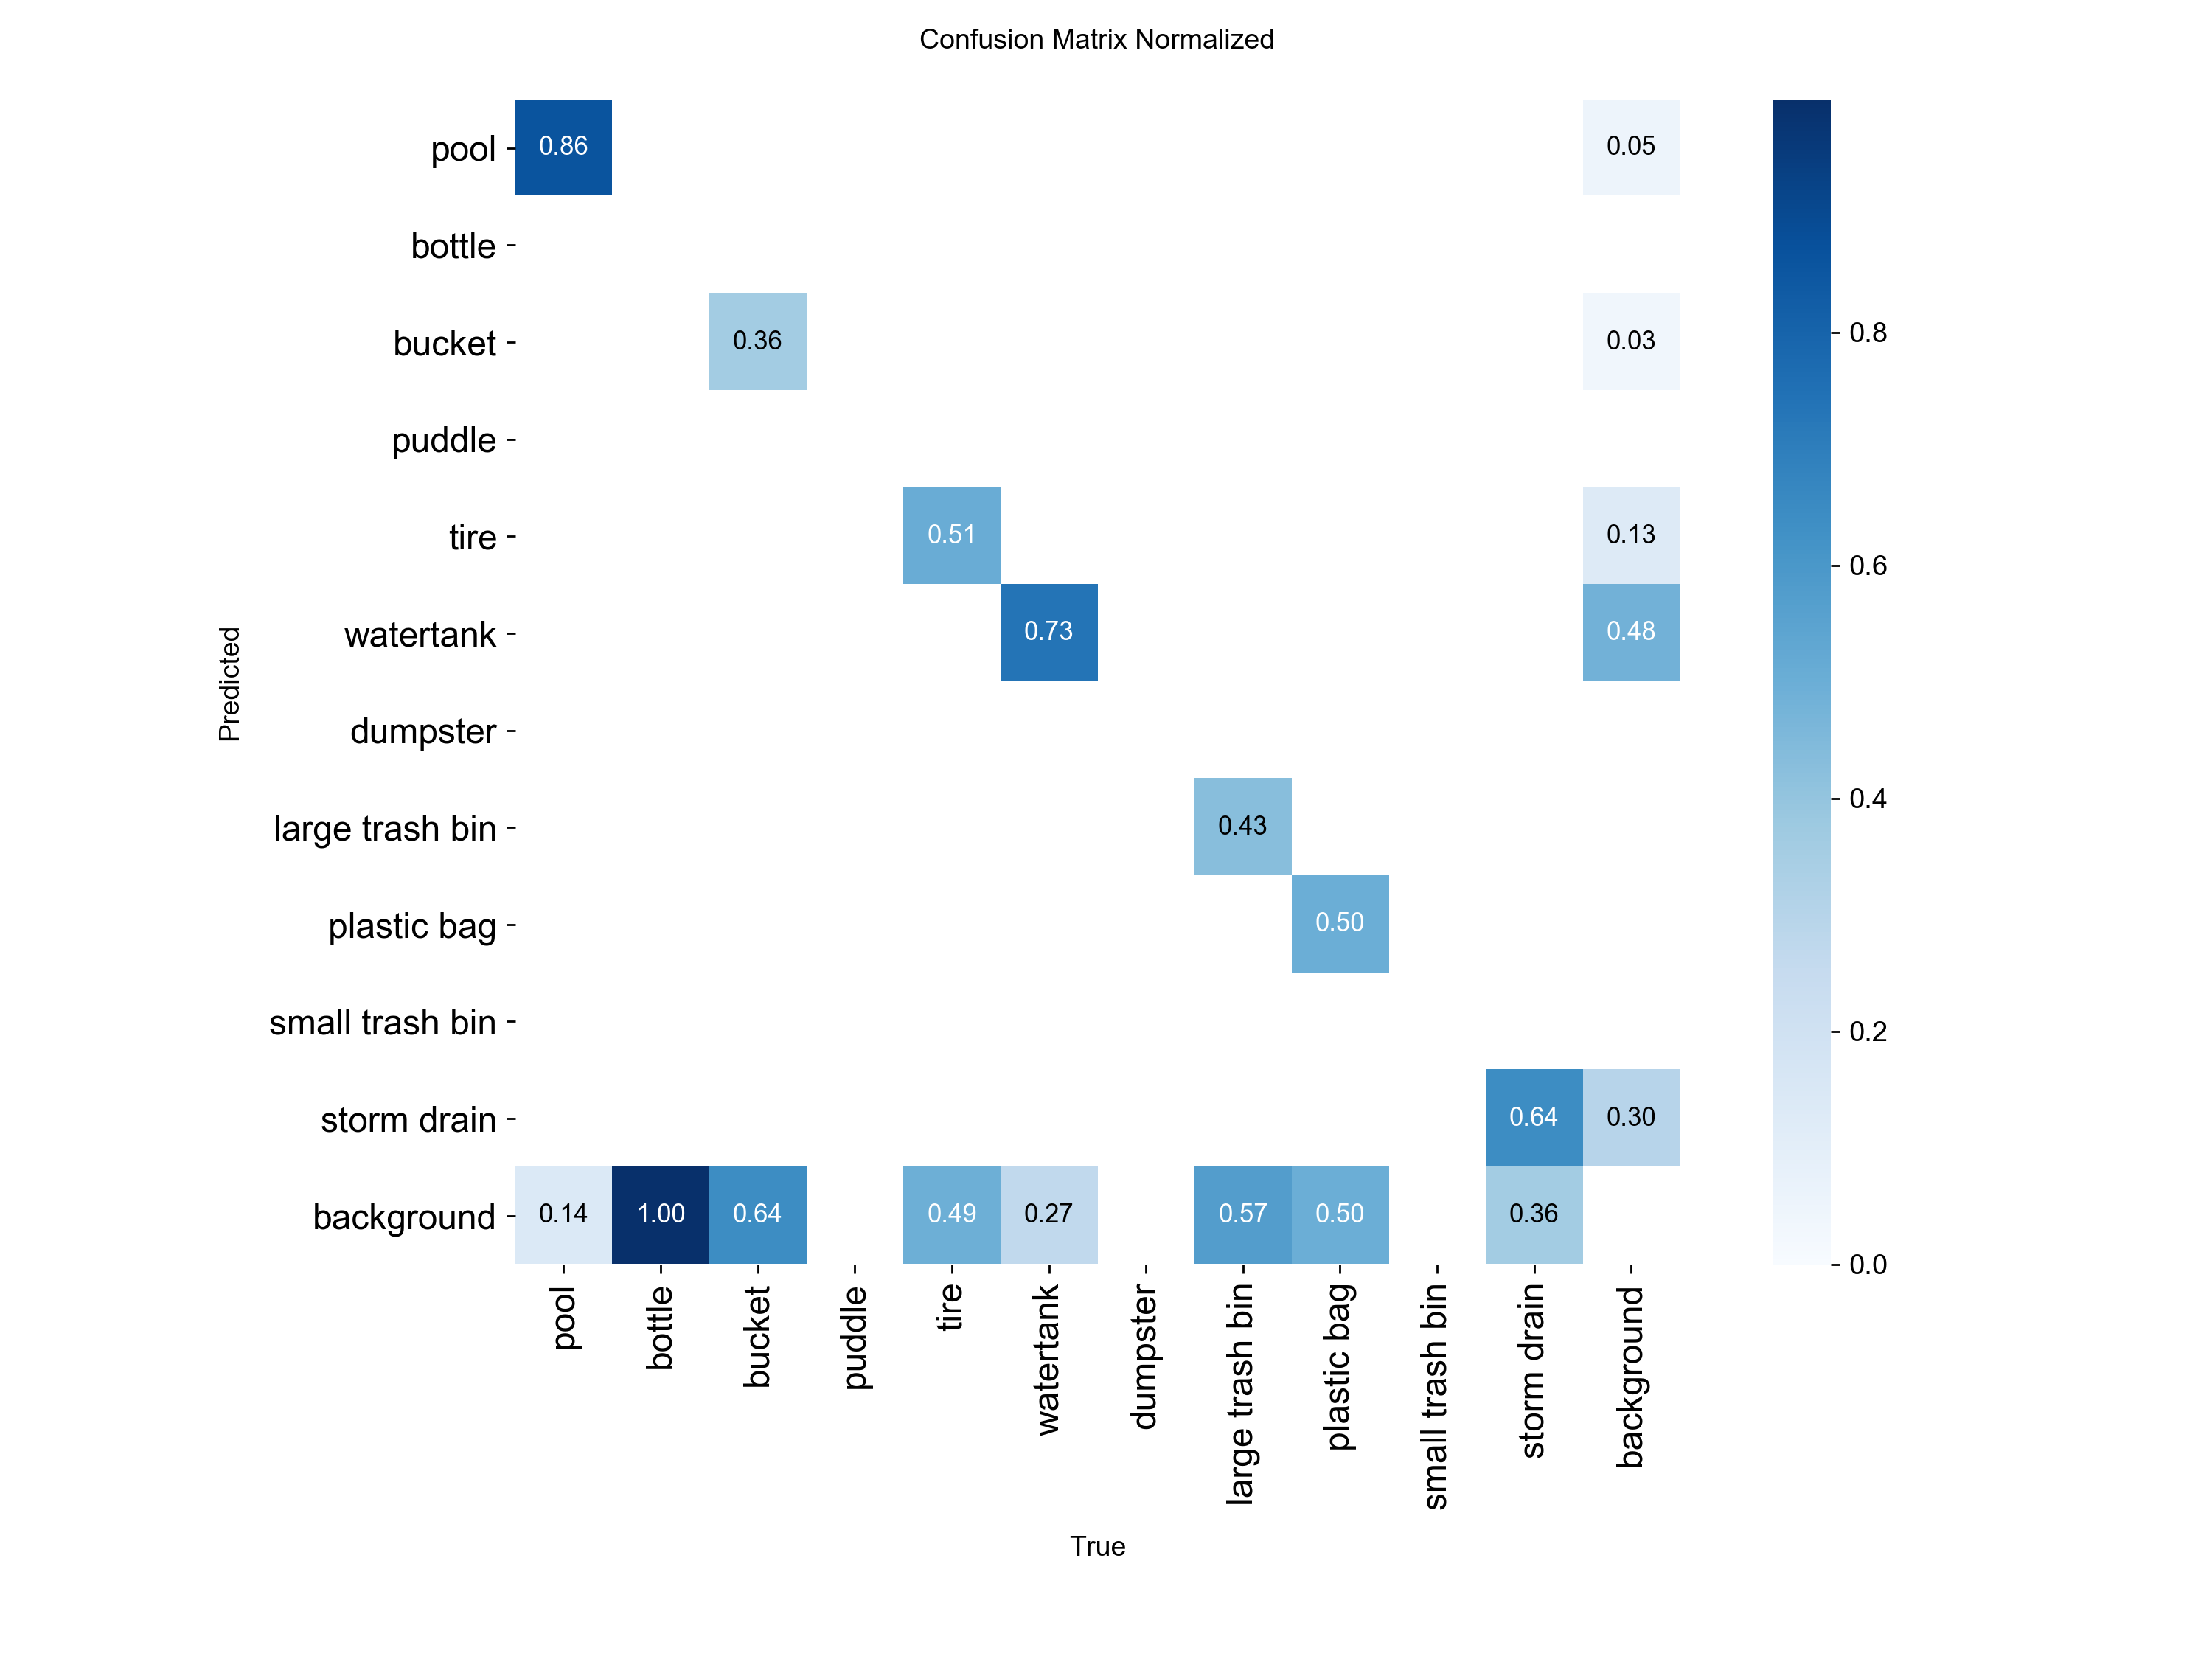
\includegraphics[width=0.9\textwidth]{figures/baseline/confusion_matrix_normalized.png}
    \caption{Normalisierte Konfusionsmatrix des Baseline-Modells. Sie verdeutlicht insbesondere die Verwechslungen seltener Klassen mit dem Hintergrund.}
    \label{fig:baseline_confusion_matrix_normalized}
\end{figure}

\subsubsection{Qualitative Validierungsbeispiele}

Zur qualitativen Kontrolle wurden zusätzlich Validierungsbeispiele betrachtet. Abbildung~\ref{fig:baseline_val_batch0} zeigt Ground-Truth-Labels und Modellvorhersagen des Baseline-Modells untereinander. Dabei wird sichtbar, dass häufige und visuell klare Klassen wie \textit{watertank} und \textit{pool} in vielen Fällen korrekt erkannt werden. Gleichzeitig treten Fehler bei kleinen Objekten und komplexen Dachstrukturen auf. Einige Objekte werden nicht erkannt, während andere Hintergrundbereiche fälschlicherweise als Objekt vorhergesagt werden.

\begin{figure}[H]
    \centering
    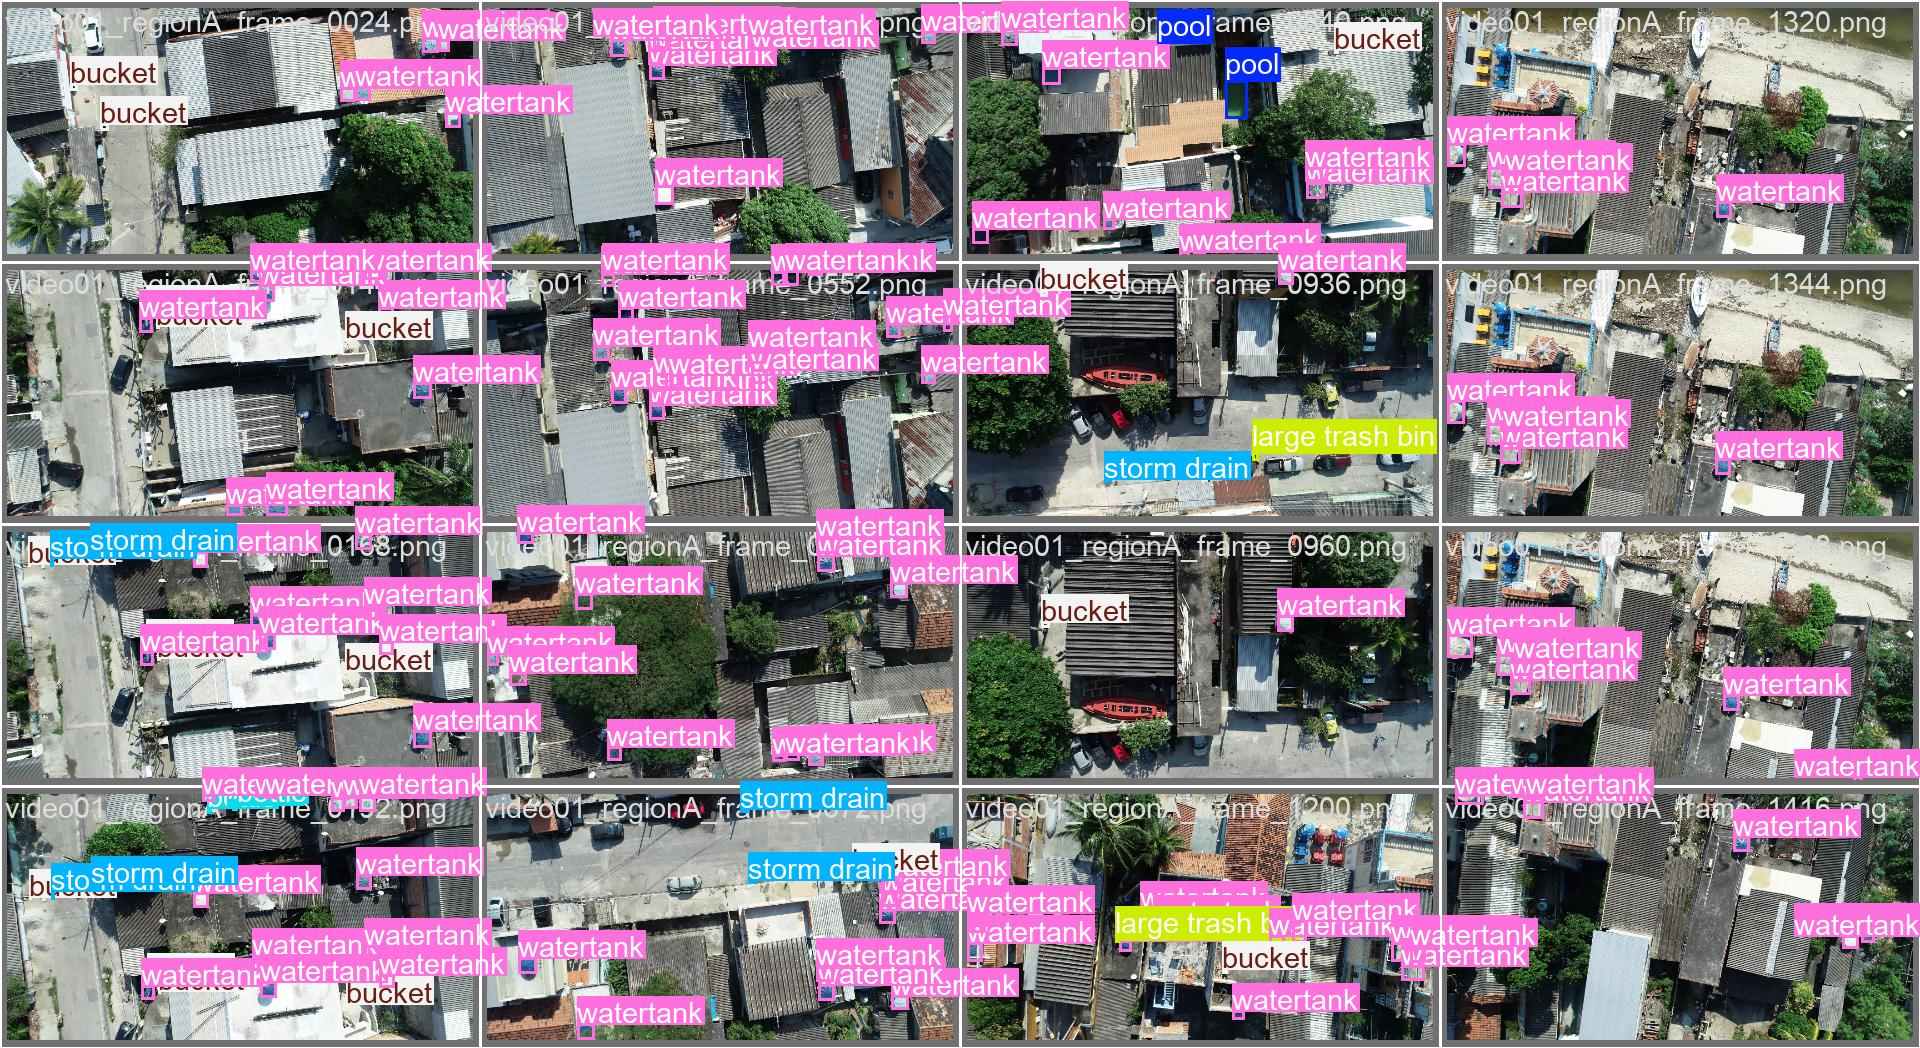
\includegraphics[width=\textwidth]{figures/baseline/val_batch0_labels.jpg}

    \vspace{0.3cm}

    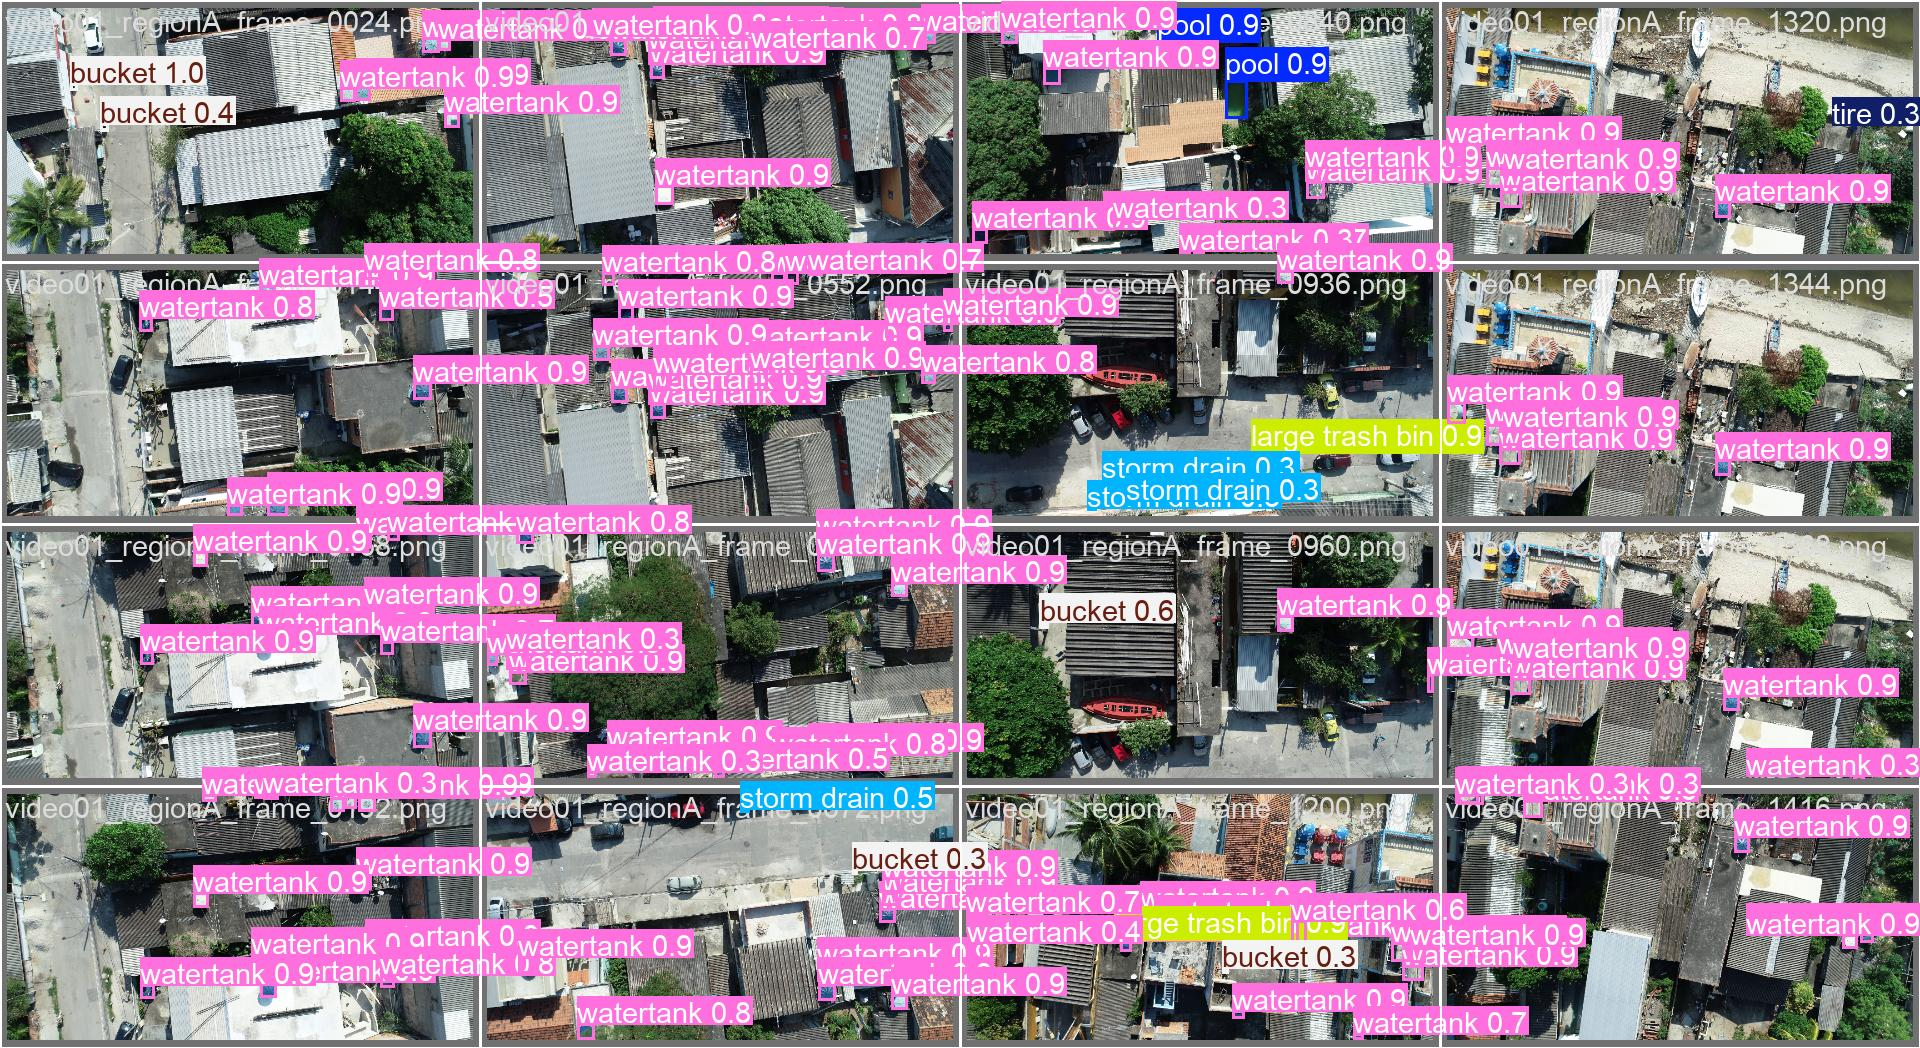
\includegraphics[width=\textwidth]{figures/baseline/val_batch0_pred.jpg}
    \caption{Qualitativer Vergleich des Baseline-Modells auf Validierungsdaten. Oben: Ground-Truth-Labels. Unten: Modellvorhersagen.}
    \label{fig:baseline_val_batch0}
\end{figure}

Zusammenfassend zeigt das Baseline-Modell eine gute Ausgangsleistung für häufige und visuell klar erkennbare Klassen, ist jedoch empfindlich gegenüber Klassenungleichgewicht, kleinen Objektgrößen und komplexen Hintergrundstrukturen.

\FloatBarrier

\subsection{Ergebnisse der automatischen Pseudo-Label-Generierung}

Auf Grundlage des Baseline-Modells wurde ein semi-supervisierter Trainingsschritt durchgeführt. Dazu wurde das zuvor trainierte Modell auf zusätzliche, nicht manuell annotierte Frames angewendet. Die dabei erzeugten Pseudo-Labels wurden zusammen mit den manuellen Annotationen in einem erweiterten Trainingsdatensatz verwendet. Ziel dieses Experiments war es, die Klassenverteilung zu verbessern und insbesondere unterrepräsentierte Klassen durch zusätzliche automatisch generierte Beispiele zu stärken.

\subsubsection{Auswirkung der Pseudo-Labels auf die Datenverteilung}

Die Label-Verteilung des erweiterten Datensatzes ist in Abbildung~\ref{fig:pseudo_labels} dargestellt. Im Vergleich zum Baseline-Datensatz ist die Verteilung mehrerer Klassen deutlich ausgeglichener. Die Anzahl der Instanzen für \textit{pool} steigt von 253 auf 743, für \textit{bucket} von 162 auf 758, für \textit{tire} von 309 auf 719, für \textit{large trash bin} von 43 auf 460 und für \textit{plastic bag} von 24 auf 534. Die Klasse \textit{watertank} bleibt mit 4432 Instanzen weiterhin die dominante Klasse, jedoch ist die extreme Ungleichverteilung im Vergleich zum Baseline-Datensatz reduziert.

\begin{figure}[htbp]
    \centering
    
\includegraphics[width=0.85\textwidth]{figures/pseudo/labels.jpg}
    \caption{Label-Verteilung nach der automatischen Pseudo-Label-Generierung. Mehrere zuvor unterrepräsentierte Klassen wurden durch zusätzliche Pseudo-Labels erweitert.}
    \label{fig:pseudo_labels}
\end{figure}

\begin{table}[htbp]
    \centering
    \caption{Vergleich der Label-Verteilung zwischen Baseline und Pseudo-Labeling}
    \label{tab:labelverteilung_baseline_pseudo}
    \begin{tabular}{lrr}
        \hline
        \textbf{Klasse} & \textbf{Baseline} & \textbf{Pseudo-Labeling} \\
        \hline
        pool            & 253               & 743                      \\
        bottle          & 14                & 14                       \\
        bucket          & 162               & 758                      \\
        puddle          & 0                 & 0                        \\
        tire            & 309               & 719                      \\
        watertank       & 4432              & 4432                     \\
        dumpster        & 4                 & 4                        \\
        large trash bin & 43                & 460                      \\
        plastic bag     & 24                & 534                      \\
        small trash bin & 14                & 14                       \\
        storm drain     & 554               & 677                      \\
        \hline
    \end{tabular}
\end{table}

\subsubsection{Auswirkung der Pseudo-Labels auf die Modellleistung}

Das semi-supervisierte Modell wurde mit dem erweiterten Datensatz erneut trainiert. Die Trainingskonfiguration verwendet das zuvor gelernte Modell als Ausgangspunkt, eine Bildgröße von 1024 Pixeln, den AdamW-Optimizer sowie eine maximale Trainingsdauer von 30 Epochen. Aufgrund der Early-Stopping-Konfiguration wurde das Training nach 12 Epochen beendet. Die Trainingskurven in Abbildung~\ref{fig:pseudo_results} zeigen, dass die Verluste weiterhin sinken, die Validierungsmetriken jedoch früh ein Plateau erreichen und stärker schwanken als beim Baseline-Modell.

\begin{figure}[htbp]
    \centering
    
\includegraphics[width=\textwidth]{figures/pseudo/results.png}
    \caption{Trainings- und Validierungsmetriken der Pseudo-Labeling-Stufe. Die Metriken zeigen eine frühe Sättigung und stärkere Schwankungen in der Validierung.}
    \label{fig:pseudo_results}
\end{figure}

Quantitativ erreicht die Pseudo-Labeling-Stufe einen mAP@50-Wert von 0{,}542 über alle Klassen. Der beste F1-Wert liegt bei 0{,}49 und wird bereits bei einem deutlich niedrigeren Confidence-Schwellenwert von 0{,}202 erreicht. In den epochbasierten Trainingsmetriken wird ein maximaler mAP@50-Wert von 0{,}561 und ein maximaler mAP@50--95-Wert von 0{,}313 erreicht. Die maximale Precision liegt bei 0{,}827, der maximale Recall bei 0{,}487.

\begin{table}[htbp]
    \centering
    \caption{Zusammenfassung der wichtigsten Kennzahlen der Pseudo-Labeling-Stufe}
    \label{tab:pseudo_kennzahlen}
    \begin{tabular}{lr}
        \hline
        \textbf{Metrik}                            & \textbf{Wert} \\
        \hline
        mAP@50, alle Klassen                       & 0{,}542       \\
        F1-Wert, alle Klassen                      & 0{,}49        \\
        optimaler Confidence-Schwellenwert         & 0{,}202       \\
        maximale Precision während des Trainings   & 0{,}827       \\
        maximaler Recall während des Trainings     & 0{,}487       \\
        maximaler mAP@50 während des Trainings     & 0{,}561       \\
        maximaler mAP@50--95 während des Trainings & 0{,}313       \\
        \hline
    \end{tabular}
\end{table}

Die Precision-Recall-Kurve der Pseudo-Labeling-Stufe ist in Abbildung~\ref{fig:pseudo_pr_curve} dargestellt. Der mAP@50-Wert über alle Klassen beträgt 0{,}542 und liegt damit nahezu auf dem Niveau des Baseline-Modells. Die klassenweise Auswertung zeigt, dass die zusätzlichen Pseudo-Labels nicht zu einer gleichmäßigen Verbesserung aller Klassen führen. Für \textit{bottle} steigt der AP@50-Wert von 0{,}461 auf 0{,}572. Dieser Wert ist jedoch aufgrund der weiterhin sehr geringen Anzahl von nur 14 Instanzen vorsichtig zu interpretieren. Geringe Verbesserungen zeigen sich außerdem bei \textit{bucket} und \textit{tire}. Gleichzeitig sinken die Werte für \textit{pool}, \textit{watertank} und insbesondere \textit{storm drain}.

\begin{figure}[htbp]
    \centering
    
\includegraphics[width=0.9\textwidth]{figures/pseudo/BoxPR_curve.png}
    \caption{Precision-Recall-Kurve der Pseudo-Labeling-Stufe. Der mAP@50-Wert über alle Klassen beträgt 0{,}542.}
    \label{fig:pseudo_pr_curve}
\end{figure}

\begin{table}[htbp]
    \centering
    \caption{Klassenweiser Vergleich der AP@50-Werte}
    \label{tab:ap_vergleich_baseline_pseudo}
    \begin{tabular}{lrrr}
        \hline
        \textbf{Klasse} & \textbf{Baseline} & \textbf{Pseudo-Labeling} & \textbf{Differenz} \\
        \hline
        pool            & 0{,}866           & 0{,}847                  & -0{,}019           \\
        bottle          & 0{,}461           & 0{,}572                  & +0{,}111           \\
        bucket          & 0{,}360           & 0{,}372                  & +0{,}012           \\
        tire            & 0{,}450           & 0{,}459                  & +0{,}009           \\
        watertank       & 0{,}737           & 0{,}707                  & -0{,}030           \\
        large trash bin & 0{,}427           & 0{,}426                  & -0{,}001           \\
        plastic bag     & 0{,}497           & 0{,}496                  & -0{,}001           \\
        storm drain     & 0{,}565           & 0{,}457                  & -0{,}108           \\
        \hline
        alle Klassen    & 0{,}545           & 0{,}542                  & -0{,}003           \\
        \hline
    \end{tabular}
\end{table}

Die F1-Confidence-Kurve der Pseudo-Labeling-Stufe ist in Abbildung~\ref{fig:pseudo_f1_curve} dargestellt. Der beste globale F1-Wert liegt bei etwa 0{,}49 und wird bei einem Confidence-Schwellenwert von 0{,}202 erreicht. Im Vergleich zum Baseline-Modell verschiebt sich der optimale Schwellenwert damit deutlich nach unten. Dies deutet darauf hin, dass das semi-supervisierte Modell mehr niedrig-konfidente Vorhersagen erzeugt und ein niedrigerer Schwellenwert notwendig ist, um den besten Kompromiss zwischen Precision und Recall zu erreichen.

\begin{figure}[htbp]
    \centering
    
\includegraphics[width=0.9\textwidth]{figures/pseudo/BoxF1_curve.png}
    \caption{F1-Confidence-Kurve der Pseudo-Labeling-Stufe. Der beste globale F1-Wert liegt bei etwa 0{,}49 bei einem Confidence-Schwellenwert von 0{,}202.}
    \label{fig:pseudo_f1_curve}
\end{figure}

Die absolute und normalisierte Konfusionsmatrix der Pseudo-Labeling-Stufe sind in Abbildung~\ref{fig:pseudo_confusion_matrix} und Abbildung~\ref{fig:pseudo_confusion_matrix_normalized} dargestellt. Die Konfusionsmatrix zeigt, dass die zusätzliche Datenmenge zwar die Klassenabdeckung verbessert, aber zugleich mehr Rauschen in den Trainingsdaten erzeugt. Besonders auffällig ist die Zunahme von False Positives für die Klasse \textit{watertank}. In der absoluten Konfusionsmatrix werden 198 Hintergrundobjekte als \textit{watertank} vorhergesagt. Auch bei \textit{storm drain} treten zusätzliche Verwechslungen mit dem Hintergrund auf. Diese Beobachtung erklärt, warum die verbesserte Klassenverteilung nicht automatisch zu einer höheren Gesamtleistung führt.

\begin{figure}[htbp]
    \centering
    
\includegraphics[width=0.9\textwidth]{figures/pseudo/confusion_matrix.png}
    \caption{Absolute Konfusionsmatrix der Pseudo-Labeling-Stufe. Auffällig ist die Zunahme von False Positives, insbesondere für die Klasse \textit{watertank}.}
    \label{fig:pseudo_confusion_matrix}
\end{figure}

\begin{figure}[htbp]
    \centering
    
\includegraphics[width=0.9\textwidth]{figures/pseudo/confusion_matrix_normalized.png}
    \caption{Normalisierte Konfusionsmatrix der Pseudo-Labeling-Stufe. Die Matrix zeigt, dass zusätzliche Pseudo-Labels auch Fehlklassifikationen verstärken können.}
    \label{fig:pseudo_confusion_matrix_normalized}
\end{figure}

Zur qualitativen Bewertung werden in Abbildung~\ref{fig:pseudo_val_batch0} Ground-Truth-Labels und Vorhersagen des Pseudo-Labeling-Modells gegenübergestellt. Die Beispiele zeigen, dass die Pseudo-Labeling-Stufe zusätzliche Objektinstanzen erkennt, jedoch auch mehr unsichere und fehlerhafte Vorhersagen erzeugt. Besonders bei \textit{watertank} treten viele Vorhersagen mit mittleren Confidence-Werten auf. Einige davon entsprechen tatsächlichen Objekten, andere liegen jedoch auf Hintergrundstrukturen wie Dächern, hellen Flächen oder runden technischen Strukturen.

\begin{figure}[H]
    \centering
    
\includegraphics[width=\textwidth]{figures/pseudo/val_batch0_labels.jpg}

    \vspace{0.3cm}

    
\includegraphics[width=\textwidth]{figures/pseudo/val_batch0_pred.jpg}
    \caption{Qualitativer Vergleich der Pseudo-Labeling-Stufe auf Validierungsdaten. Oben: Ground-Truth-Labels. Unten: Modellvorhersagen.}
    \label{fig:pseudo_val_batch0}
\end{figure}

Insgesamt zeigt dieses Experiment, dass die automatische Pseudo-Label-Generierung grundsätzlich geeignet ist, die Datenbasis zu erweitern und unterrepräsentierte Klassen stärker abzudecken. Gleichzeitig wird deutlich, dass ungefilterte oder nur schwach gefilterte Pseudo-Labels Fehler des Ausgangsmodells in den erweiterten Trainingsdatensatz übertragen können. Dadurch entsteht eine Form von Rauschverstärkung, die insbesondere bei kleinen Objekten, komplexen Dachstrukturen und visuell ähnlichen Hintergrundbereichen sichtbar wird.

\FloatBarrier

\subsection{Ergebnisse der tracking-basierten Label-Propagation}

Ziel dieses Experiments war nicht die erneute Optimierung des Detektionsmodells, sondern die qualitative Bewertung der Tracking-Leistung im Hinblick auf eine konsistente Objektverfolgung über mehrere aufeinanderfolgende Frames. Da die Objektverfolgung direkt auf den UAV-Videosequenzen durchgeführt wurde, erfolgt die Bewertung anhand repräsentativer Frame-Sequenzen. Dadurch lässt sich untersuchen, ob erkannte Objekte trotz Kamerabewegung und wechselnder Perspektiven über mehrere Frames hinweg konsistent verfolgt werden können.

\subsubsection{Tracking-Auswertung}

Nach Abschluss der Objekterkennung wurde die Tracking-Komponente auf die vollständige UAV-Videosequenz angewendet. Während dieses Prozesses wurde zusätzlich ein automatischer Tracking-Bericht erzeugt, der statistische Informationen über die verarbeiteten Frames, die Anzahl der Detektionen sowie die erzeugten Objekttracks enthält. Diese Auswertung dient als quantitative Zusammenfassung der Tracking-Ausführung und ergänzt die anschließende qualitative Analyse.

\begin{table}[htbp]
    \centering
    \caption{Zusammenfassung der Tracking-Auswertung über die gesamte Videosequenz}
    \label{tab:tracking_summary}
    \begin{tabular}{lr}
        \hline
        \textbf{Kennzahl}       & \textbf{Wert} \\
        \hline
        Verarbeitete Frames     & 6285          \\
        Detektionen insgesamt   & 51\,867       \\
        Eindeutige Objekttracks & 716           \\
        \hline
    \end{tabular}
\end{table}

Insgesamt wurden 6285 Frames verarbeitet und dabei 51\,867 Objektdetektionen erzeugt. Diese wurden durch das Tracking-Verfahren zu 716 eindeutigen Objekttracks zusammengeführt. Die Ergebnisse zeigen, dass das Verfahren auch bei langen UAV-Videosequenzen eine kontinuierliche Zuordnung wiederkehrender Objekte ermöglicht.

\subsubsection{Klassenbezogene Tracking-Statistik}

Neben den Gesamtkennzahlen liefert der Tracking-Bericht eine klassenbezogene Aufschlüsselung der Detektionen und der erzeugten Objekttracks. Tabelle~\ref{tab:tracking_classstats} fasst diese Werte zusammen.

\begin{table}[htbp]
    \centering
    \caption{Klassenbezogene Tracking-Statistik der ausgewerteten Videosequenz}
    \label{tab:tracking_classstats}
    \begin{tabular}{lrr}
        \hline
        \textbf{Klasse} & \textbf{Detektionen} & \textbf{Tracks} \\
        \hline
        watertank       & 42\,135              & 498             \\
        pool            & 4\,147               & 47              \\
        storm drain     & 2\,682               & 68              \\
        tire            & 1\,284               & 33              \\
        bucket          & 1\,011               & 75              \\
        plastic bag     & 608                  & 3               \\
        \hline
    \end{tabular}
\end{table}

Die Klassenstatistik zeigt deutliche Unterschiede zwischen den Objektklassen. Die Klasse \textit{watertank} dominiert sowohl hinsichtlich der Anzahl der Detektionen als auch der erzeugten Objekttracks. Seltene Klassen wie \textit{plastic bag} erzeugen dagegen nur wenige stabile Tracks. Dieses Verhalten entspricht der zuvor beobachteten Klassenverteilung des Datensatzes und bestätigt, dass häufig vertretene Klassen robuster verfolgt werden können.

\subsubsection{Qualitative Analyse}

Abbildung~\ref{fig:tracking_sequence} zeigt zwei aufeinanderfolgende Frames derselben Videosequenz. Trotz der kontinuierlichen Bewegung der Drohne behalten mehrere Objekte ihre Track-ID über beide Frames hinweg bei. Beispielsweise werden die Objekte der Klasse \textit{pool} mit den Track-IDs 14, 18 und 19 sowie die Objekte der Klasse \textit{watertank} mit den IDs 1, 4 und 8 in beiden Frames konsistent erkannt und verfolgt. Die gleichbleibenden Track-IDs zeigen, dass das eingesetzte Tracking-Verfahren die Zuordnung derselben Objekte über aufeinanderfolgende Frames zuverlässig aufrechterhalten kann.

\begin{figure}[H]
    \centering

    \begin{subfigure}{0.49\textwidth}
        \centering
        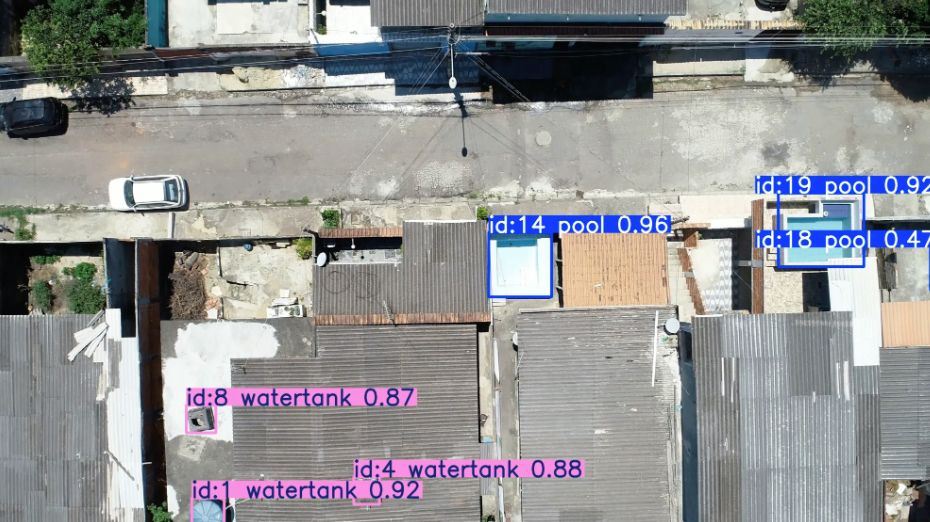
\includegraphics[width=\linewidth]{figures/tracking/tracking_frame1.jpeg}
        \caption{Frame $t$}
    \end{subfigure}
    \hfill
    \begin{subfigure}{0.49\textwidth}
        \centering
        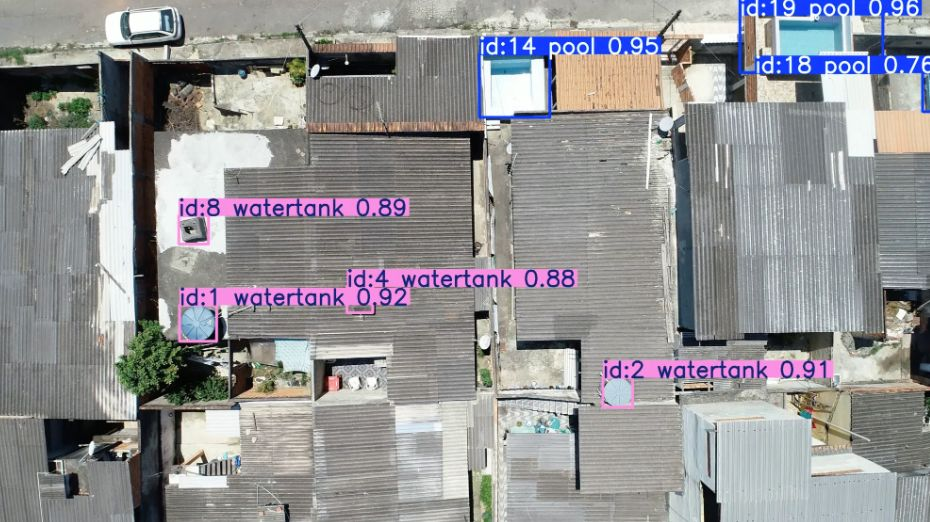
\includegraphics[width=\linewidth]{figures/tracking/tracking_frame2.jpeg}
        \caption{Frame $t+1$}
    \end{subfigure}

    \caption{Zwei aufeinanderfolgende Frames derselben Videosequenz. Trotz der Kamerabewegung behalten mehrere Objekte ihre Track-ID über beide Frames hinweg bei. Dies verdeutlicht die zeitliche Konsistenz der tracking-basierten Objektverfolgung.}
    \label{fig:tracking_sequence}
\end{figure}

Darüber hinaus zeigt die Sequenz, dass neue Track-IDs entstehen können, wenn Objekte erstmals in den sichtbaren Bildbereich eintreten oder zuvor aufgrund der Kameraperspektive nicht eindeutig detektiert werden konnten. Im gezeigten Beispiel erscheint zusätzlich ein weiterer \textit{watertank}, der als neuer Track initialisiert wird. Dieses Verhalten entspricht dem erwarteten Arbeitsprinzip moderner Multi-Object-Tracking-Verfahren und stellt keinen Trackingfehler dar.

Die Ergebnisse verdeutlichen, dass die Kombination aus Objekterkennung und Tracking insbesondere bei Videodaten einen zusätzlichen Mehrwert gegenüber einer rein framebasierten Betrachtung bietet. Während einzelne Detektionen zwischen benachbarten Frames geringfügig in ihrer Position oder Konfidenz variieren können, ermöglicht die konsistente Zuordnung derselben Track-ID eine stabile zeitliche Verknüpfung wiederkehrender Objekte. Dadurch können automatisch erzeugte Annotationen über mehrere Frames hinweg nachvollzogen und qualitativ überprüft werden.

Für die automatische Annotation bedeutet dies, dass Tracking nicht als eigenständiger zusätzlicher Trainingsschritt eingesetzt wird, sondern als unterstützende Komponente zur Analyse der zeitlichen Konsistenz automatisch erzeugter Detektionen dient. Insbesondere bei UAV-Videodaten liefert die kontinuierliche Objektverfolgung zusätzliche Informationen, die mit einer rein framebasierten Auswertung nicht verfügbar wären.

\FloatBarrier

\subsection{Vergleich der experimentellen Stufen}

Der direkte Vergleich zwischen Baseline-Modell und Pseudo-Labeling-Stufe zeigt, dass die Erweiterung des Datensatzes durch automatisch erzeugte Labels die Klassenverteilung deutlich verbessert, jedoch nicht zu einer klaren Verbesserung der Detektionsleistung führt. Der mAP@50-Wert bleibt nahezu unverändert. Während das Baseline-Modell einen mAP@50-Wert von 0{,}545 erreicht, liegt die Pseudo-Labeling-Stufe bei 0{,}542. Der globale F1-Wert sinkt von 0{,}53 auf 0{,}49.

\begin{table}[htbp]
    \centering
    \caption{Vergleich der bisher ausgewerteten experimentellen Stufen}
    \label{tab:vergleich_experimentelle_stufen}
    \begin{tabular}{lrr}
        \hline
        \textbf{Metrik}                    & \textbf{Baseline} & \textbf{Pseudo-Labeling} \\
        \hline
        mAP@50                             & 0{,}545           & 0{,}542                  \\
        F1-Wert                            & 0{,}53            & 0{,}49                   \\
        optimaler Confidence-Schwellenwert & 0{,}462           & 0{,}202                  \\
        maximale Precision                 & ca. 0{,}85        & 0{,}827                  \\
        maximaler Recall                   & ca. 0{,}53        & 0{,}487                  \\
        \hline
    \end{tabular}
\end{table}

Da für die tracking-basierte Stufe keine eigenständige quantitative Auswertung auf demselben Validierungssplit vorliegt, fasst Tabelle~\ref{tab:vergleich_alle_stufen} alle drei experimentellen Stufen zusammen. Die Übersicht stellt bewusst nicht ausschließlich auf mAP-Werte ab, sondern unterscheidet zwischen quantitativ und qualitativ ausgewerteten Stufen und benennt die jeweils zentrale Beobachtung.

\begin{table}[H]
    \centering
    \caption{Vergleich der experimentellen Stufen}
    \label{tab:vergleich_alle_stufen}
    \begin{tabular}{p{3.3cm}p{3.3cm}p{2.1cm}p{3.6cm}}
        \hline
        \textbf{Stufe}                      & \textbf{Datengrundlage}         & \textbf{Bewertung} & \textbf{Zentrale Beobachtung}                                   \\
        \hline
        Baseline-Modell                     & Manuelle Annotationen           & Quantitativ        & Solide Leistung bei häufigen Klassen, begrenzter Recall         \\
        Pseudo-Labeling                     & Manuelle Labels + Pseudo-Labels & Quantitativ        & Verbesserte Klassenabdeckung, aber zusätzliche Fehlannotationen \\
        Tracking-basierte Label-Propagation & Detektionen über Videoframes    & Qualitativ         & Stabilisierung wiederkehrender Detektionen über die Zeit        \\
        \hline
    \end{tabular}
\end{table}

Diese Ergebnisse zeigen, dass die reine Erhöhung der Label-Anzahl nicht ausreichend ist, um die Modellleistung zuverlässig zu verbessern. Entscheidend ist nicht nur die Menge zusätzlicher Labels, sondern auch deren Qualität. Werden fehlerhafte Pseudo-Labels in den Trainingsprozess übernommen, kann das Modell falsche Zuordnungen verstärken. Dies zeigt sich insbesondere an der Zunahme von False Positives für \textit{watertank} sowie an der schlechteren Leistung für \textit{storm drain}.

Gleichzeitig liefert die Pseudo-Labeling-Stufe einen wichtigen experimentellen Befund: Automatisch erzeugte Labels können die Abdeckung unterrepräsentierter Klassen verbessern. Für einen produktiven Einsatz ist jedoch eine zusätzliche Qualitätskontrolle erforderlich, beispielsweise durch höhere Confidence-Schwellenwerte, klassenabhängige Filterregeln, manuelle Stichprobenkontrolle oder eine Kombination mit tracking-basierter zeitlicher Konsistenzprüfung.

\subsection{Qualitative Analyse}

Die qualitativen Beispiele aus Abbildung~\ref{fig:baseline_val_batch0} und Abbildung~\ref{fig:pseudo_val_batch0} bestätigen die quantitativen Ergebnisse. In vielen Validierungsbildern erkennt das Modell häufige und visuell klare Klassen wie \textit{watertank} und \textit{pool} zuverlässig. Besonders Pools sind aufgrund ihrer Farbe, Form und räumlichen Abgrenzung vergleichsweise gut unterscheidbar. Auch größere Wassertanks auf Dächern werden in vielen Fällen korrekt lokalisiert.

Gleichzeitig zeigen die Validierungsbeispiele typische Fehlerfälle. Auf dicht bebauten Dachflächen werden kleine helle oder runde Strukturen teilweise fälschlicherweise als \textit{watertank} erkannt. Dies führt zu einer erhöhten Anzahl von False Positives. Zudem werden kleine Objekte wie \textit{plastic bag}, \textit{bottle} oder \textit{large trash bin} nicht stabil erkannt, da sie häufig nur wenige Pixel groß sind und sich visuell kaum vom Hintergrund unterscheiden. Bei \textit{storm drain} treten Verwechslungen mit dunklen rechteckigen Hintergrundstrukturen auf, insbesondere auf Straßen oder an Dachrändern.

Die Pseudo-Label-Beispiele zeigen außerdem, dass automatisch erzeugte Labels häufig mit mittleren Confidence-Werten auftreten. Solche Labels können nützlich sein, wenn sie korrekt sind und zusätzliche Objektvariationen abdecken. Gleichzeitig besteht jedoch das Risiko, dass unsichere Vorhersagen als Trainingsdaten übernommen werden. Dies ist vor allem dann problematisch, wenn ein falsch erkanntes Objekt in mehreren ähnlichen Frames erneut als Pseudo-Label erzeugt wird. In diesem Fall kann sich der Fehler im erweiterten Datensatz wiederholen.

Die qualitative Analyse macht daher deutlich, dass Pseudo-Labeling allein nicht ausreicht, um eine robuste automatische Annotation sicherzustellen. Besonders bei UAV-Videodaten mit kleinen Objekten, hoher Hintergrundkomplexität und stark unausgewogenen Klassen ist eine zusätzliche Stabilisierung notwendig. Hier bietet die tracking-basierte Label-Propagation einen sinnvollen nächsten Schritt, da sie Einzelvorhersagen über mehrere Frames hinweg prüfen und zeitlich konsistentere Labels erzeugen kann.

\subsection{Diskussion der Ergebnisse}

Die bisher durchgeführten Experimente zeigen, dass ein YOLO-basiertes Detektionsmodell auch mit sparsam annotierten UAV-Frames relevante Objektklassen lernen kann. Das Baseline-Modell erreicht für häufige Klassen wie \textit{pool} und \textit{watertank} gute Ergebnisse, während seltene Klassen und kleine Objekte deutlich schwieriger zu erkennen sind. Die stark unausgewogene Klassenverteilung stellt dabei eine zentrale Einschränkung dar.

Die automatische Pseudo-Label-Generierung reduziert diese Ungleichverteilung teilweise. Insbesondere die Klassen \textit{pool}, \textit{bucket}, \textit{tire}, \textit{large trash bin} und \textit{plastic bag} erhalten durch den semi-supervisierten Schritt deutlich mehr Trainingsbeispiele. Dennoch führt diese Erweiterung nicht zu einer klaren Verbesserung der Gesamtleistung. Der mAP@50-Wert bleibt nahezu konstant, während der F1-Wert leicht sinkt. Dies zeigt, dass die zusätzlichen Pseudo-Labels zwar die Datenmenge erhöhen, aber zugleich Rauschen in den Trainingsprozess einbringen.

Die Ergebnisse verdeutlichen damit eine zentrale Herausforderung semi-supervisierter Annotation: Die Qualität der automatisch erzeugten Labels ist entscheidend. Ein Modell, das auf einem unausgewogenen Datensatz trainiert wurde, kann seine eigenen Fehler in den Pseudo-Labels reproduzieren. Werden diese Labels ohne ausreichende Kontrolle erneut zum Training verwendet, können False Positives und Klassenverwechslungen verstärkt werden. Dies ist besonders bei Klassen problematisch, die visuell ähnlich zum Hintergrund sind oder nur in geringer Anzahl vorkommen.

Aus methodischer Sicht spricht dies für eine stärker kontrollierte Pseudo-Label-Auswahl. Möglich sind höhere oder klassenabhängige Confidence-Schwellenwerte, eine Begrenzung der maximalen Anzahl automatisch erzeugter Labels pro Klasse, eine manuelle Kontrolle besonders unsicherer Pseudo-Labels sowie die Nutzung zeitlicher Konsistenz durch Tracking. Gerade bei Videodaten ist die zeitliche Struktur ein wichtiger Vorteil gegenüber Einzelbildern. Ein Objekt, das über mehrere aufeinanderfolgende Frames stabil erkannt wird, ist mit höherer Wahrscheinlichkeit ein korrektes Label als eine isolierte Einzelvorhersage.

Zusammenfassend zeigen die Experimente, dass der vorgeschlagene Ansatz grundsätzlich geeignet ist, den manuellen Annotierungsaufwand zu reduzieren. Das Baseline-Modell liefert eine brauchbare Ausgangsbasis, und die Pseudo-Labeling-Stufe verbessert die Klassenabdeckung deutlich. Gleichzeitig zeigen die Ergebnisse, dass Pseudo-Labels sorgfältig gefiltert und idealerweise durch Tracking stabilisiert werden müssen, um eine tatsächliche Verbesserung der Detektionsleistung zu erreichen.
